\chapter{\textit{Análise dinâmica e Controle Mini Parrot}}

Nos capítulos anteriores construímos uma base teórica sobre dinâmica e controle de um quadricóptero, assim, nesse capítulo vamos relacionar o que foi dito nos capítulos anteriores com o sistema de controle desenvolvido pela MathWorks em parceria com a parrot para fins de estudo. 

O sistema de controle já desenvolvido é bem completo e complexo, então nossa intenção será avaliar as características do sistema de controle durante um voo pairado e verificar a possibilidade de implementar melhorias no sistema.

\section{Características do quadricóptero}

O quadricóptero selecionado foi o Parrot Mambo Fly, esse é um drone pequeno(18 x 18 x 4 cm), e leve (~68 gramas). O quadricóptero utiliza uma configuração de rotores em "X", onde o eixo X do sistema de referência do corpo é alinhado entre os dois rotores frontais, diferente deê um drone com configuração em "+" onde o eixo x aponta diretamente para o rotor frontal. Cada rotor têm um motor de corrente continua sem escovas. Além disso o quadricóptero tem autonomia entre 8 e 10 minutos, a partir de uma bateria de litio de 660mAh. A memória interna do drone é de 1GB, e ele tem um processador com velocidade de 200Hz. O drone também conta com alguns sensores que são utilizados para o controle, são eles:

- Camera: Uma cãmera de 0.3 megapixel, que fica na parte de baixo do drone, com uma taxa de quadros de 60 fps. Utilizada para medir o deslocamento horizontal do drone com o método de fluxo ótico, que consiste em estimar a velocidade baseada no movimento relativo entre os quadros.

- Ultrasom: O sensor ultrasônico, localizado também na parte debaixo do drone, mede a posição vertical do drone relativo ao solo, ou seja, mede a altitude. A faixa de operação desse sensor é de 4 metros. 

- Sensor de Pressão: É utilizado para medir a altitude do drone, quando essa for maior do que 4 metros(faixa de operação do sensor ultrasônico), utilizando-se do fato que a pressão atmosférica é inversamente proporcional a altitude.

- IMU: Composta por um acelerômetro de 3 eixos que mede a aceleração linear e um giroscópio de 3 eixos para medição da velocidade angular.

Como já dissemos o drone tem uma configuração em "X", e é importante notar que os motores opostos rotacionam na mesma direção, mas na direção inversa do outro par. Isso é necessário para que possamos controlar, a propulsão, a rolagem, a guinada e a arfagem de maneira independente(apesar do fato que existe acoplamento entre os movimentos, mas para os nosso propósito vamos desconsiderá-los).

Agora que já temos noção das características do nosso drone, vamos analisar o sistema de controle desenvolvido pela MathWorks para testes e simulações com o Parrot Mambo minidrone.

\section{O projeto do quadricóptero no Matlab Simulink}

Primeiramente para abrir o projeto no matlab, temos que rodar o comando \textit{asbQuadcopterStart}, iniciando assim o projeto. Onde podemos ver todos os componentes que compõe o sistema de controle. 

\begin{figure}[H]
	\centering
	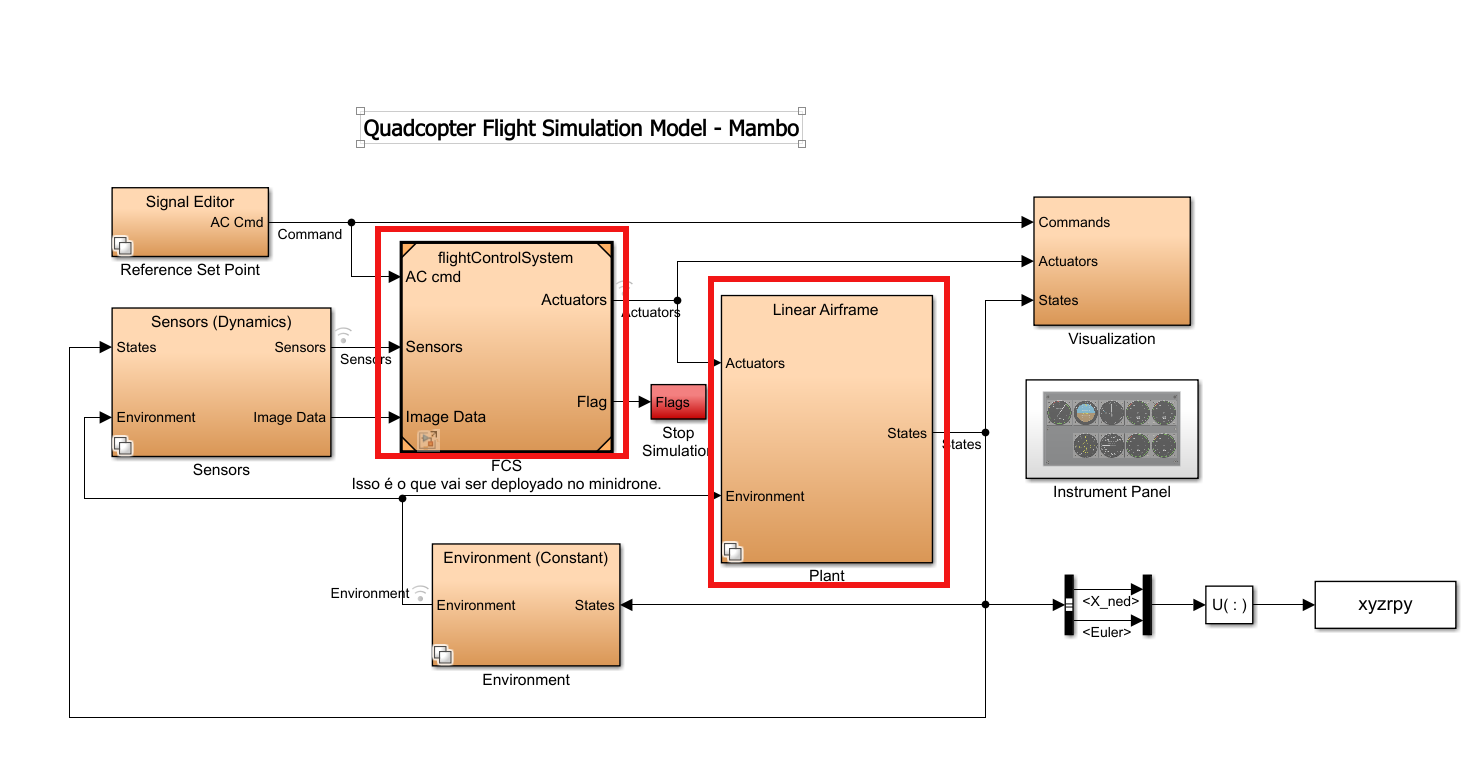
\includegraphics[width=0.6\textwidth]{asbQuadcopterProject}
	\caption{Modelo de Voo do Quadricóptero Parrot Mambo}
	\centering
	\label{Modelo de Voo do Quadricóptero Parrot Mambo}
\end{figure}

Não é o foco desse trabalho analisar todos os componentes desse modelo,analisaremos apenas os componentes em destque na figura, vamos focar no Sistema de Controle de Voo, que é o nosso controlador(recebe as medidas dos sensores e calcula o input para a planta, além disso pode ser implantado no drone), e na planta que é o modelo físico do nosso drone. Entretantom falaremos brevemente sobre os outros componentes.

Reference Set Point - Define qual tipo de entrada será usada como comando, temos 4 opções, joystick(controle remoto), sinais(entradas temporais), dados em função do tempo em um arquivo .mat ou .xlsx.

Sensors - Os sensores que a partir de suas medidas vão calcular o estado atual das nossas variáveis de interesse.

Environment - É uma constante que define se nas simulações será usado um modelo constante de ambiente externo(gravidade constante, pressão constante, etc), ou um modelo dinâmico, onde esses valores variam de acordo com a altura e posição.

Visualization - Construído para para extrair e apresentar os dados de voo e possui 4 formas de visualização, além de extrair os dados necessários para o "Instrument Panel"

Instrument Panel - Painel instrumentado para visualização de alguns dados de voo.

\subsection{Sistema de Controle de Voo}

\begin{figure}[H]
	\centering
	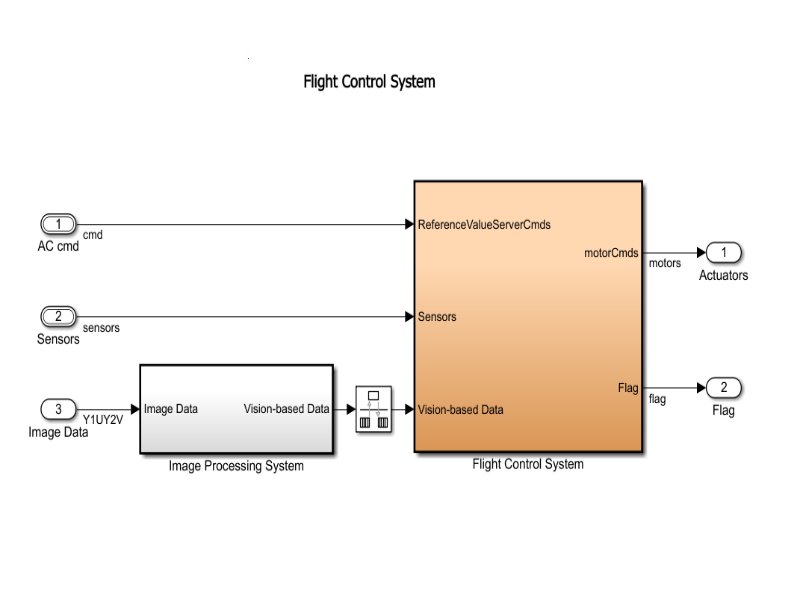
\includegraphics[width=0.6\textwidth]{flightControlSystem}
	\caption{Modelo do sistema de controle de voo}
	\centering
	\label{flightControlSystem}
\end{figure}

Na arquitetura definida pela parrot no simulink, podemos observar que o controlador recebe os valores de referência dos comandos, os dados dos sensores(menos da câmera), e os dados da câmera separadamente. E seus parâmetros de saída são os comandos para os motores atingirem a posição desejada e um parâmetro para prevenção de batidas acidentais. Assim, na sequência vamos adrentar no bloco principal da imagem acima(Flight Control System), e entender seu funcionamento.


\begin{figure}[H]
	\centering
	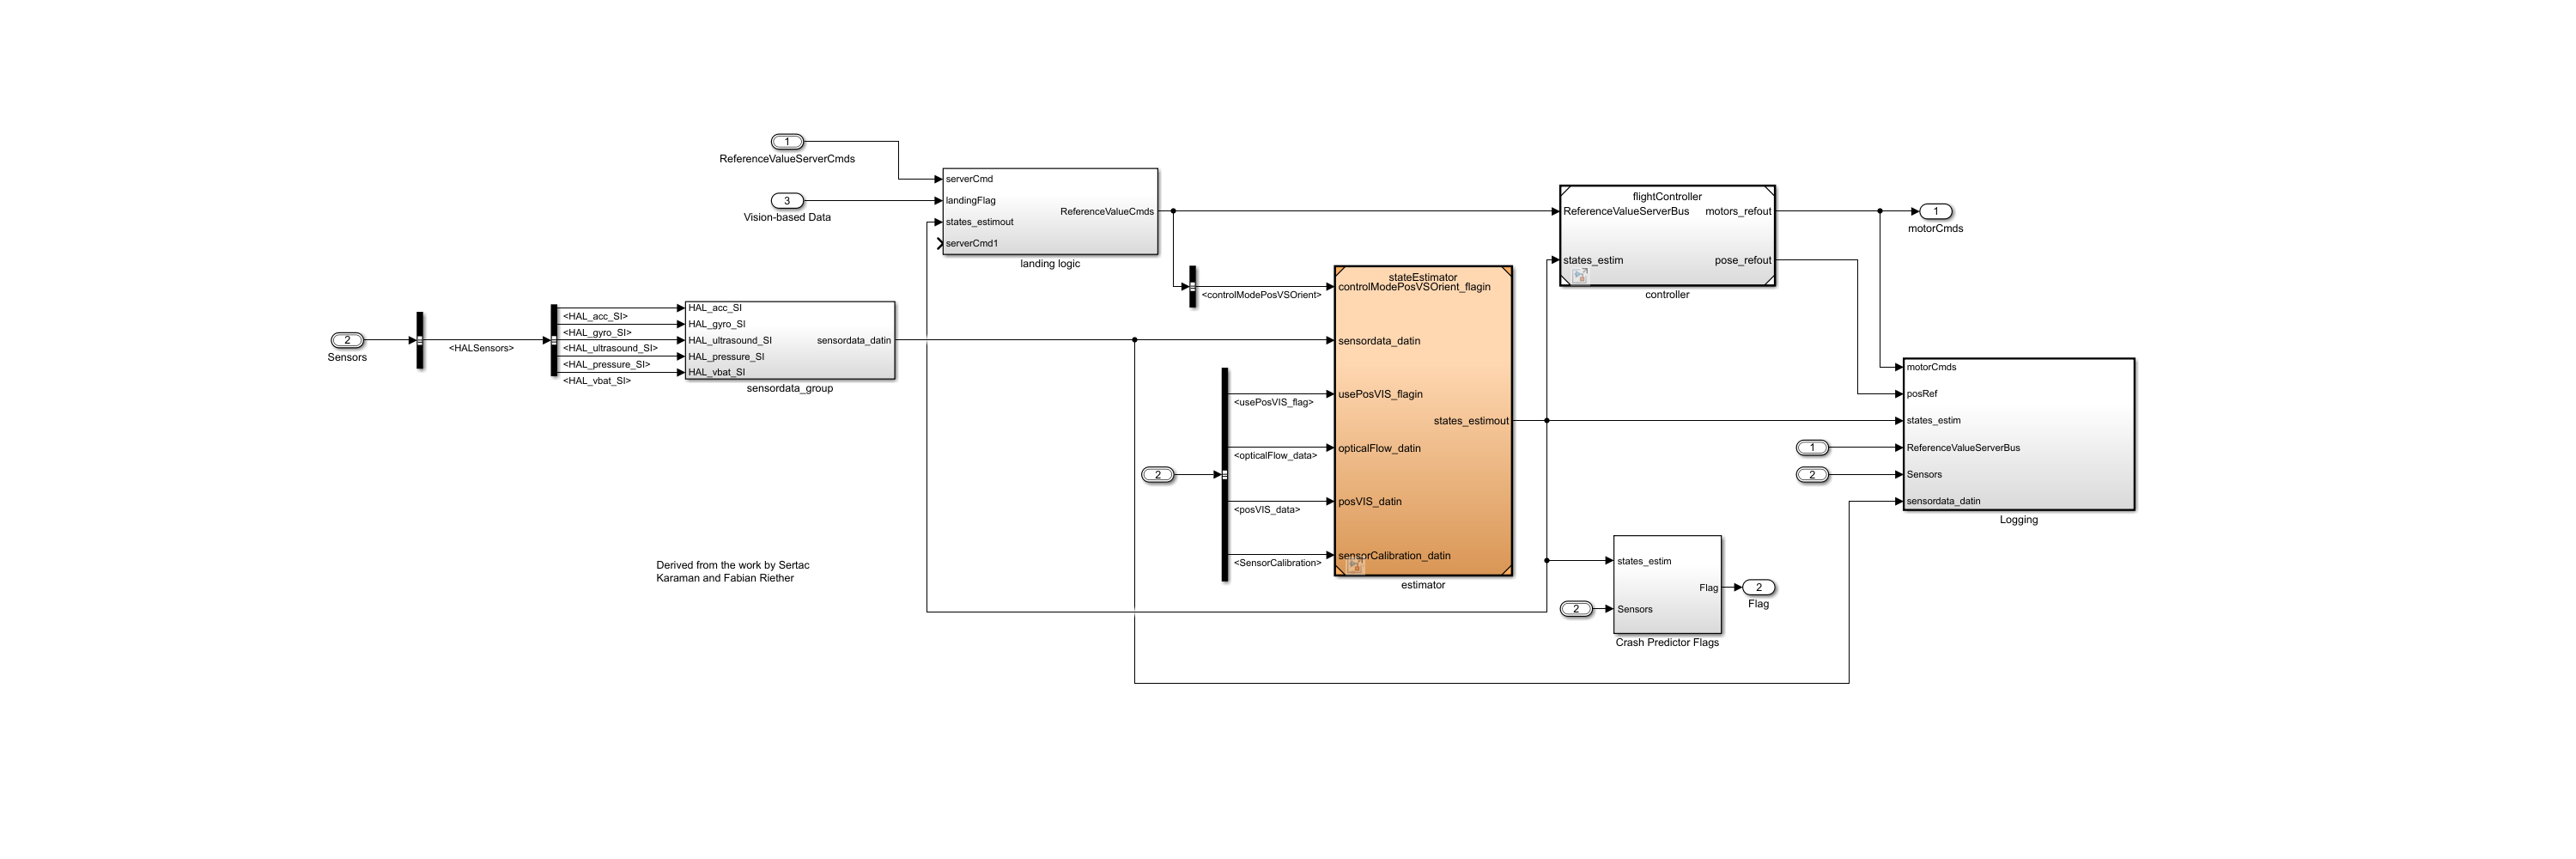
\includegraphics[width=1\textwidth]{flightControlSystem-inside}
	\caption{Dentro do Sistema de controle de Voo}
	\centering
	\label{flightControlSystem-inside}
\end{figure}


Aqui podemos ver alguns blocos importantes:

- Sensor Data Group: Agrup os dados dos sensores de forma mais adequada para ser usada durante o restante do fluxo, como podemos ver na imagem abaixo.

\begin{figure}[H]
	\centering
	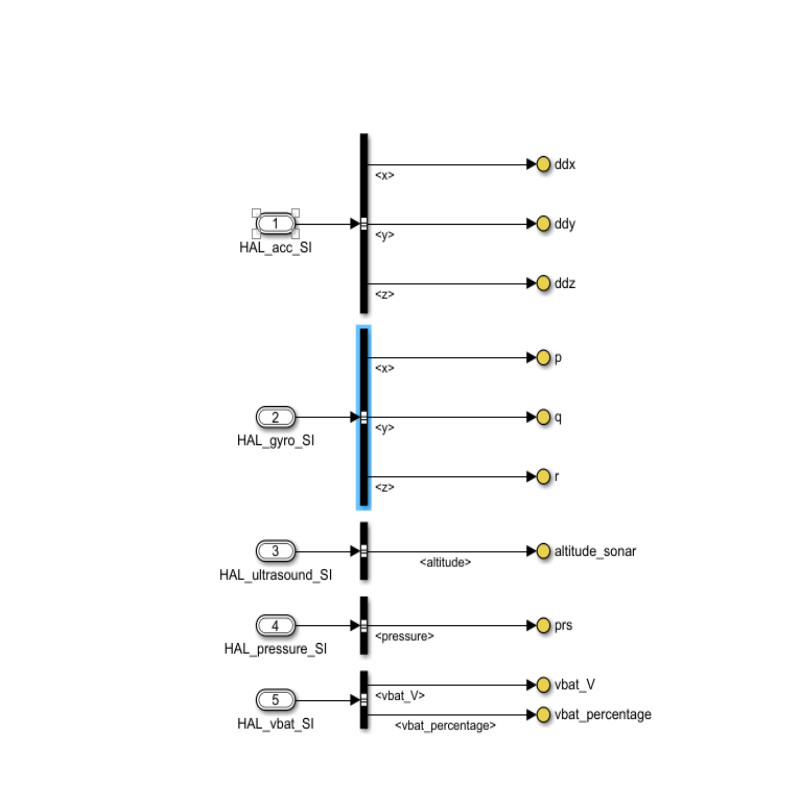
\includegraphics[width=1\textwidth]{flightControlSystem-sensordatagroup}
	\caption{Agrupamento de dados dos sensores}
	\centering
	\label{flightControlSystem-sensordatagroup}
\end{figure}

- Landing Logic - Contém a lógica para um pouso controlado, vamos falar mais sobre ela em breve com o intuito de utiliza-lá para simulações. 

- Estimator - É o estimador de estado do nosso sistema de controle, ele recebe basicamente todos os dados coletados pelos sensores e agrupados a partir do "Sensor Data Group",os dados de calibração desses sensores, além dos dados coletados da câmera a partir da técnica de fluco ótico(optical flow). Com o intuito de estimar o estado completo do quadricóptero, ou seja sua posição X,Y,Z, sua velocidade dx, dy, dz e sua orientação, ângulo rolagem($\phi$), arfagem($\phi$) e guinad($\psi$), e também a orientação do corpo no sistema de referência do corpo.
Olhando dentro do estimador de estados, podemos ver alguns blocos importantes:

-Sensor Pré-Processing: Pré processa os dados dos sensores, e valida alguns dados das câmeras para saber se podem ser utilizados.

-Complementary Filter: Filtro complementar com o intuito de combinar os diferentes sensores e obter medições mais precisas, da orientação do quadricóptero.

-Estimator XY Position: Responsável por estimar as posições XY, além das velocidades nesses eixos. 

-Estimator Altitude: Responsável por estimar a posição no eixo Z e sua respectiva velocidade.

\begin{figure}[H]
	\centering
	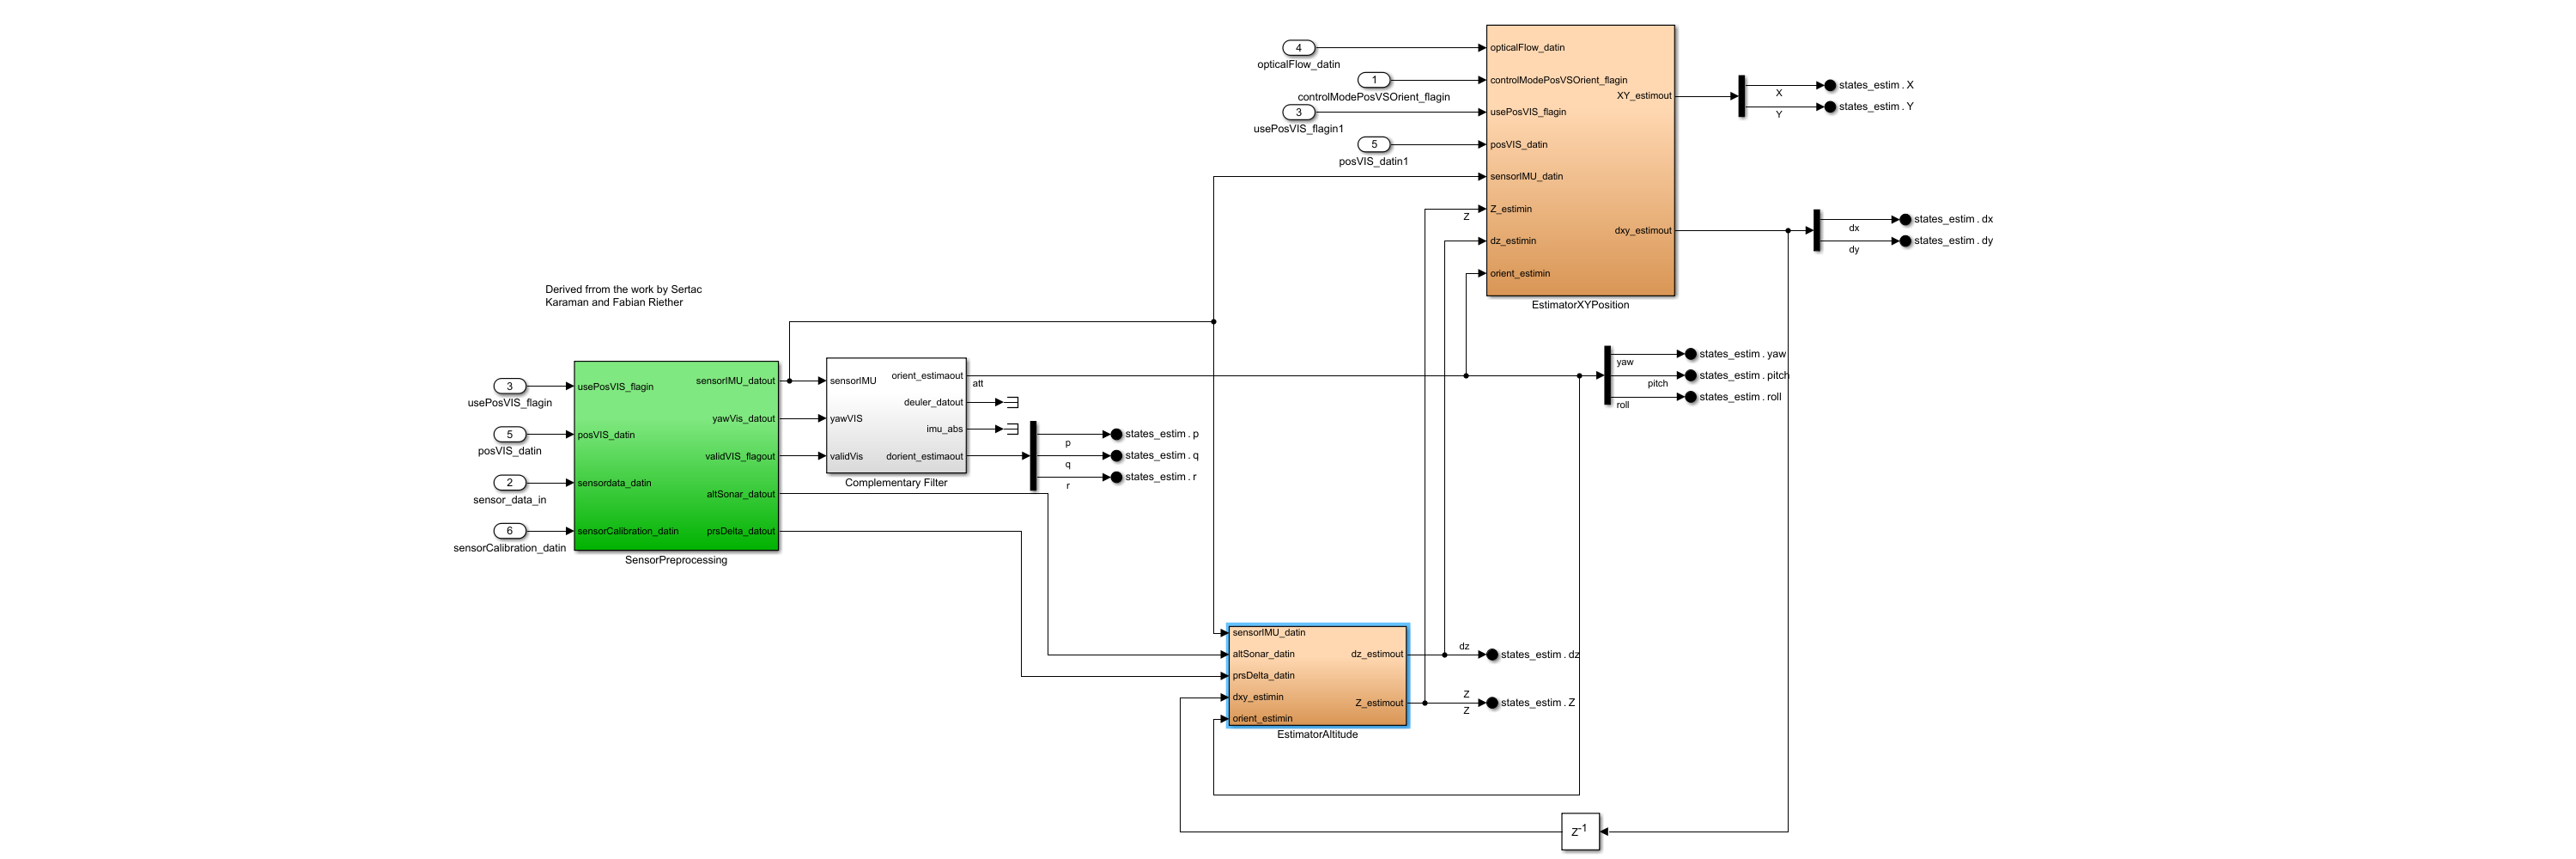
\includegraphics[width=1\textwidth]{flightControlSystem-estateestimator}
	\caption{Estimador de Estados}
	\centering
	\label{Estimador de Estados}
\end{figure}

A seguir ainda dentro do sistema de controle de voo, vamos entrar dentro do bloco do controlador, que é um dos blocos de interesse nesse trabalho.

\subsection{Controlador}

Olhando dentro do controlador, temos blocos importantes e que ainda serão explorados nesse trabalho afim de fazer melhorias no sistema de controle existente, por hora vamos apenas explica o que há em cada um dos blocos e como eles interagem entre si. 


\begin{figure}[H]
	\centering
	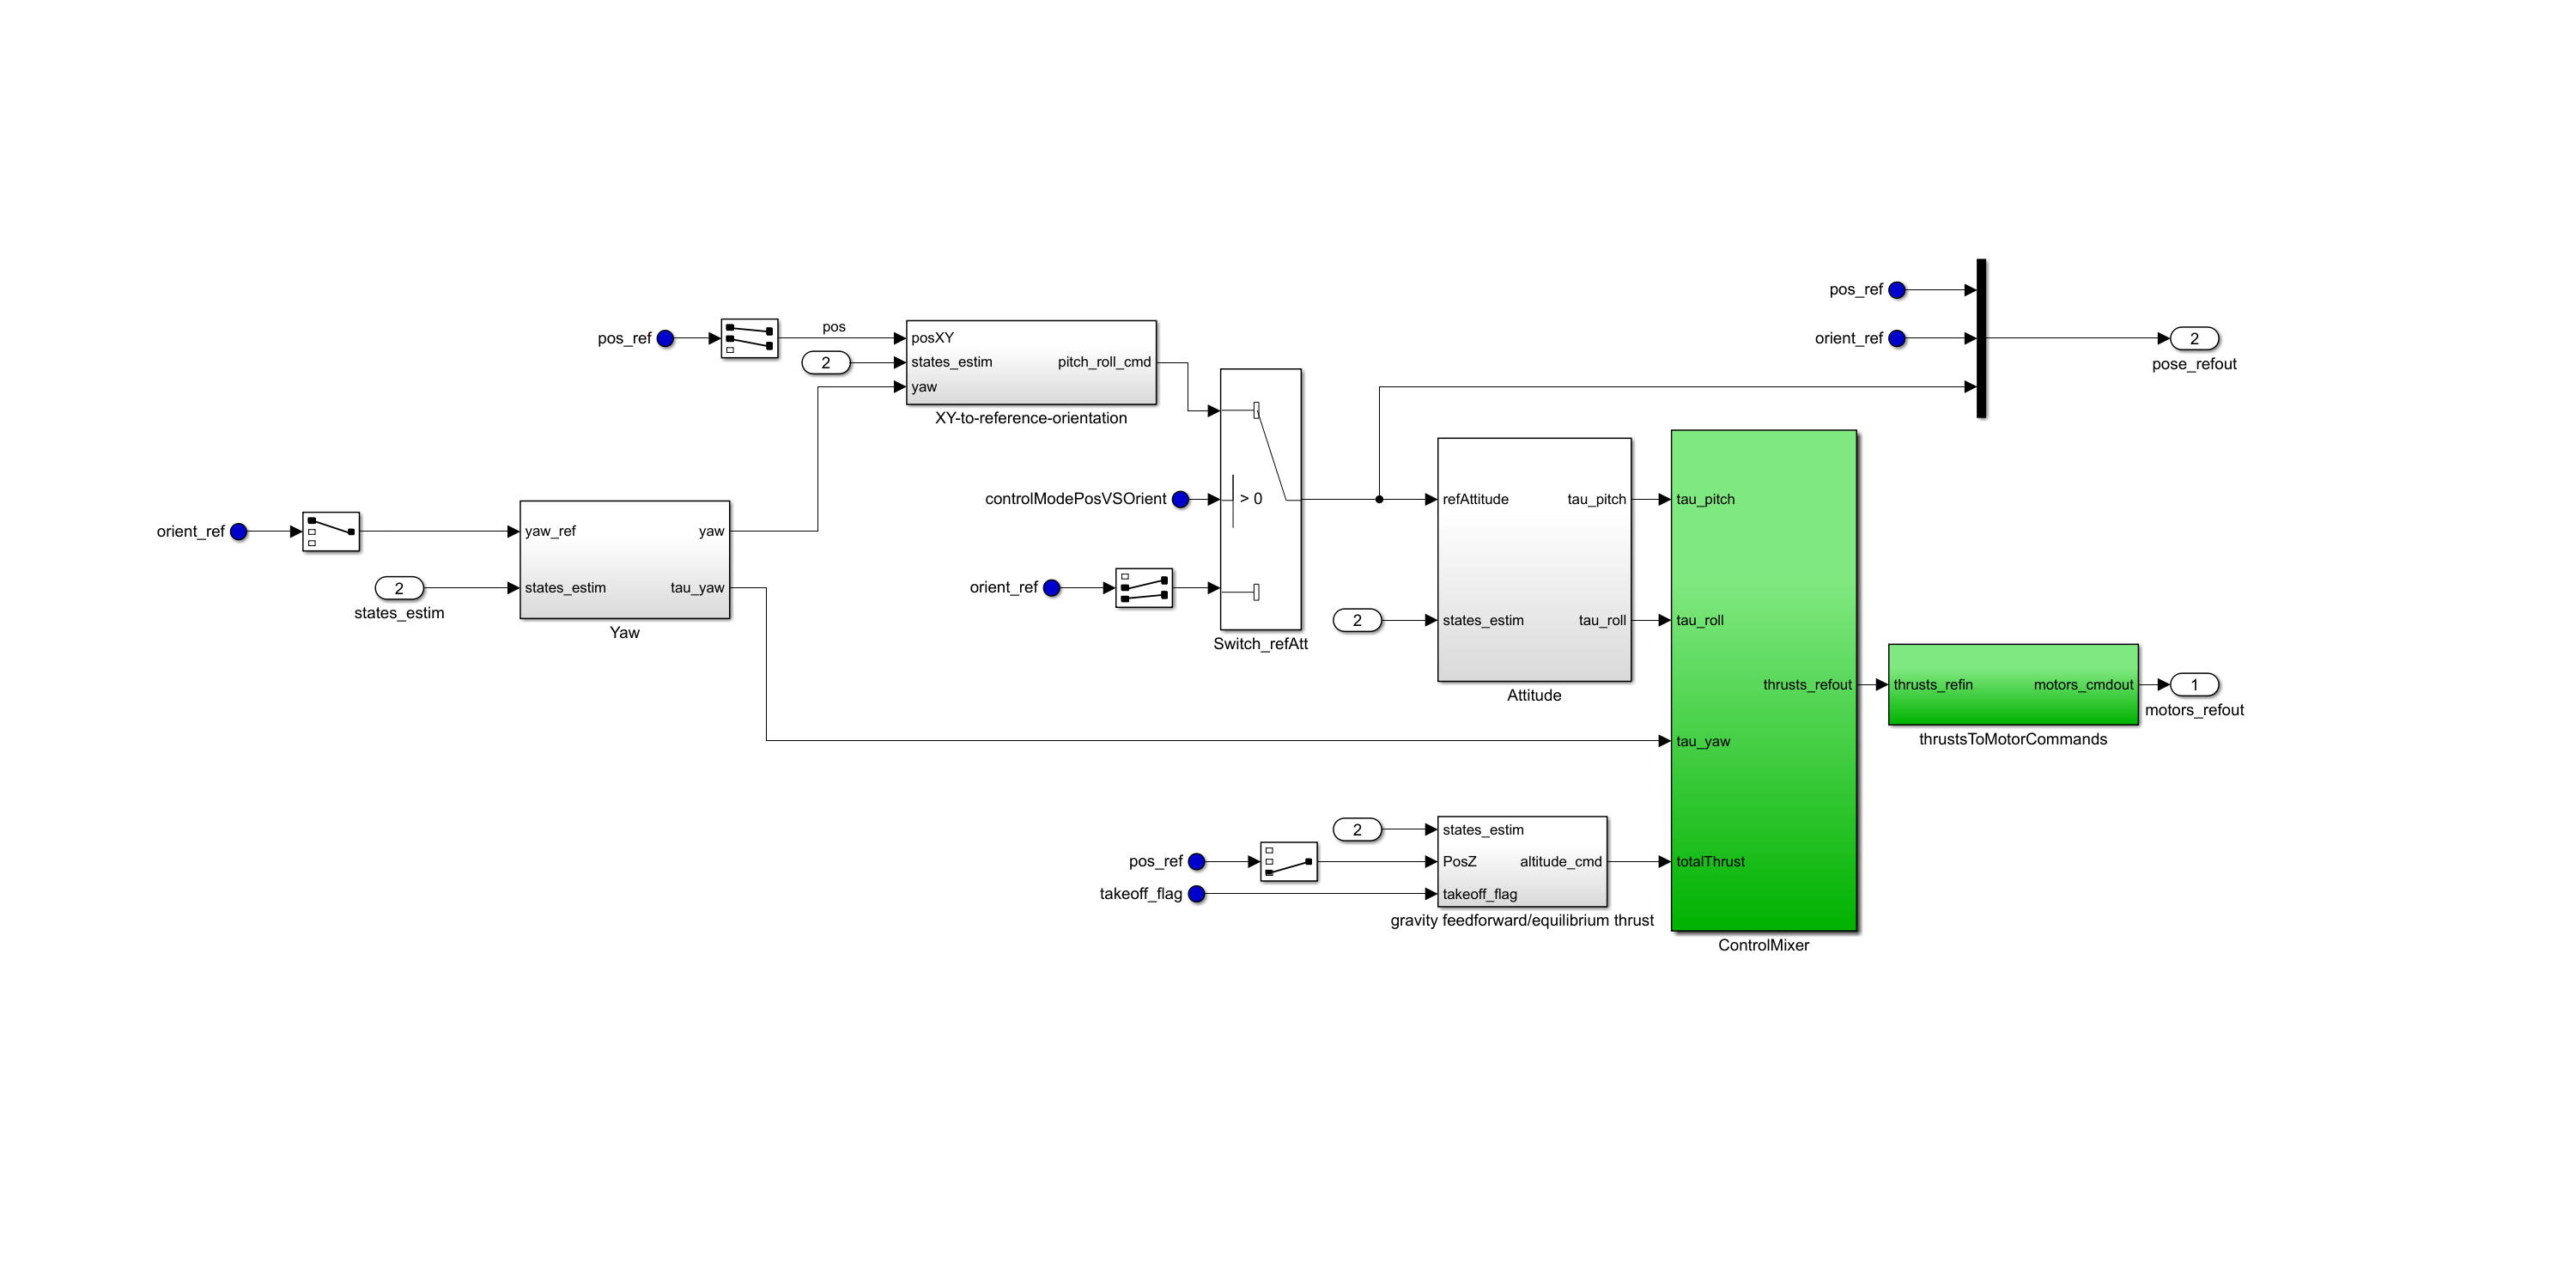
\includegraphics[width=0.8\textwidth]{flightControlSystem-controller}
	\caption{Controlador}
	\centering
	\label{Controlador}
\end{figure}

-Yaw - Controlador de guinada, tem o objetivo de calcular o torque necessário para que o quadricóptero atinja sua posição de guinada desejada. Faz isso através de um controlado PD, como podemos ver na imagem abaixo. Como o movimento de guinada não sofre influência ou sofre pouca influência dos movimentos de rolamento e arfagem, tem um controlador independente.

\begin{figure}[H]
	\centering
	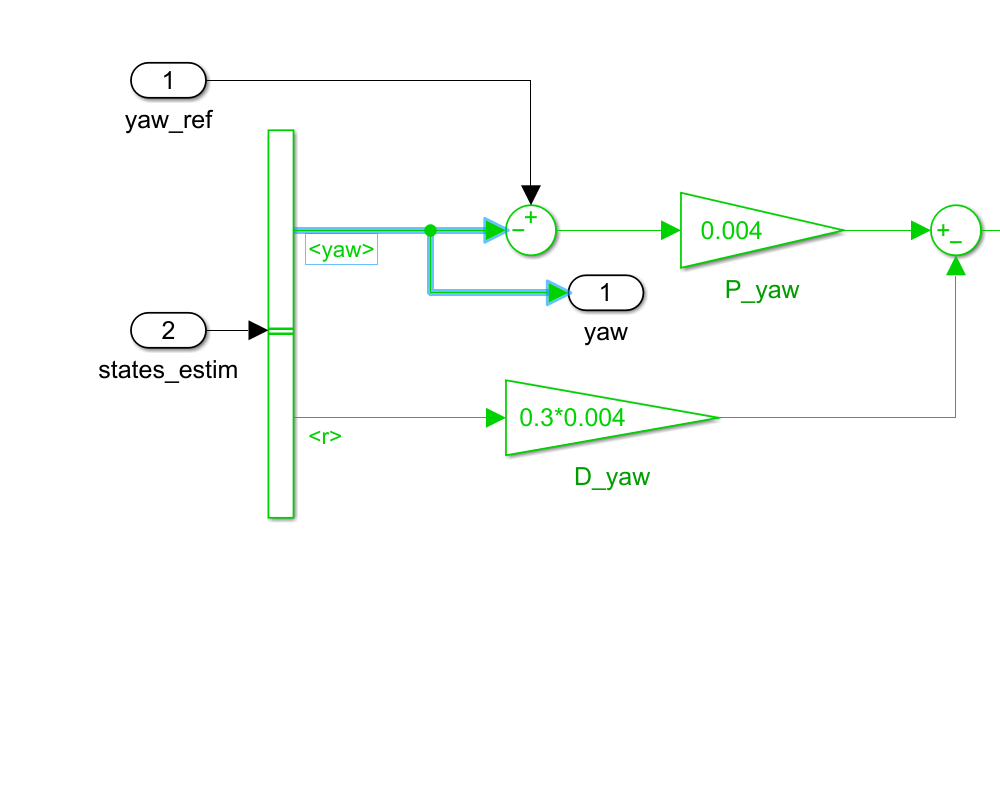
\includegraphics[width=0.8\textwidth]{flightControlSystem-controller-yaw}
	\caption{Controlador de Guinada}
	\centering
	\label{Controlador de Guinada}
\end{figure}

-XY to Reference Position - Tem o papel de calcular a atitude(angulo de rolamento e de arfagem) de referência do quadricóptero a partir da posição no plano XY e suas respectivas velocidades nessse plano, entretanto nem sempre esse calculo é usado, podemos ver que existe um bloco "switch", que valida se o valor é maior que zero, e caso não seja utiliza a orientação de referência calculada pelo estimador de estados que já foi falado anteriormente.

\begin{figure}[H]
	\centering
	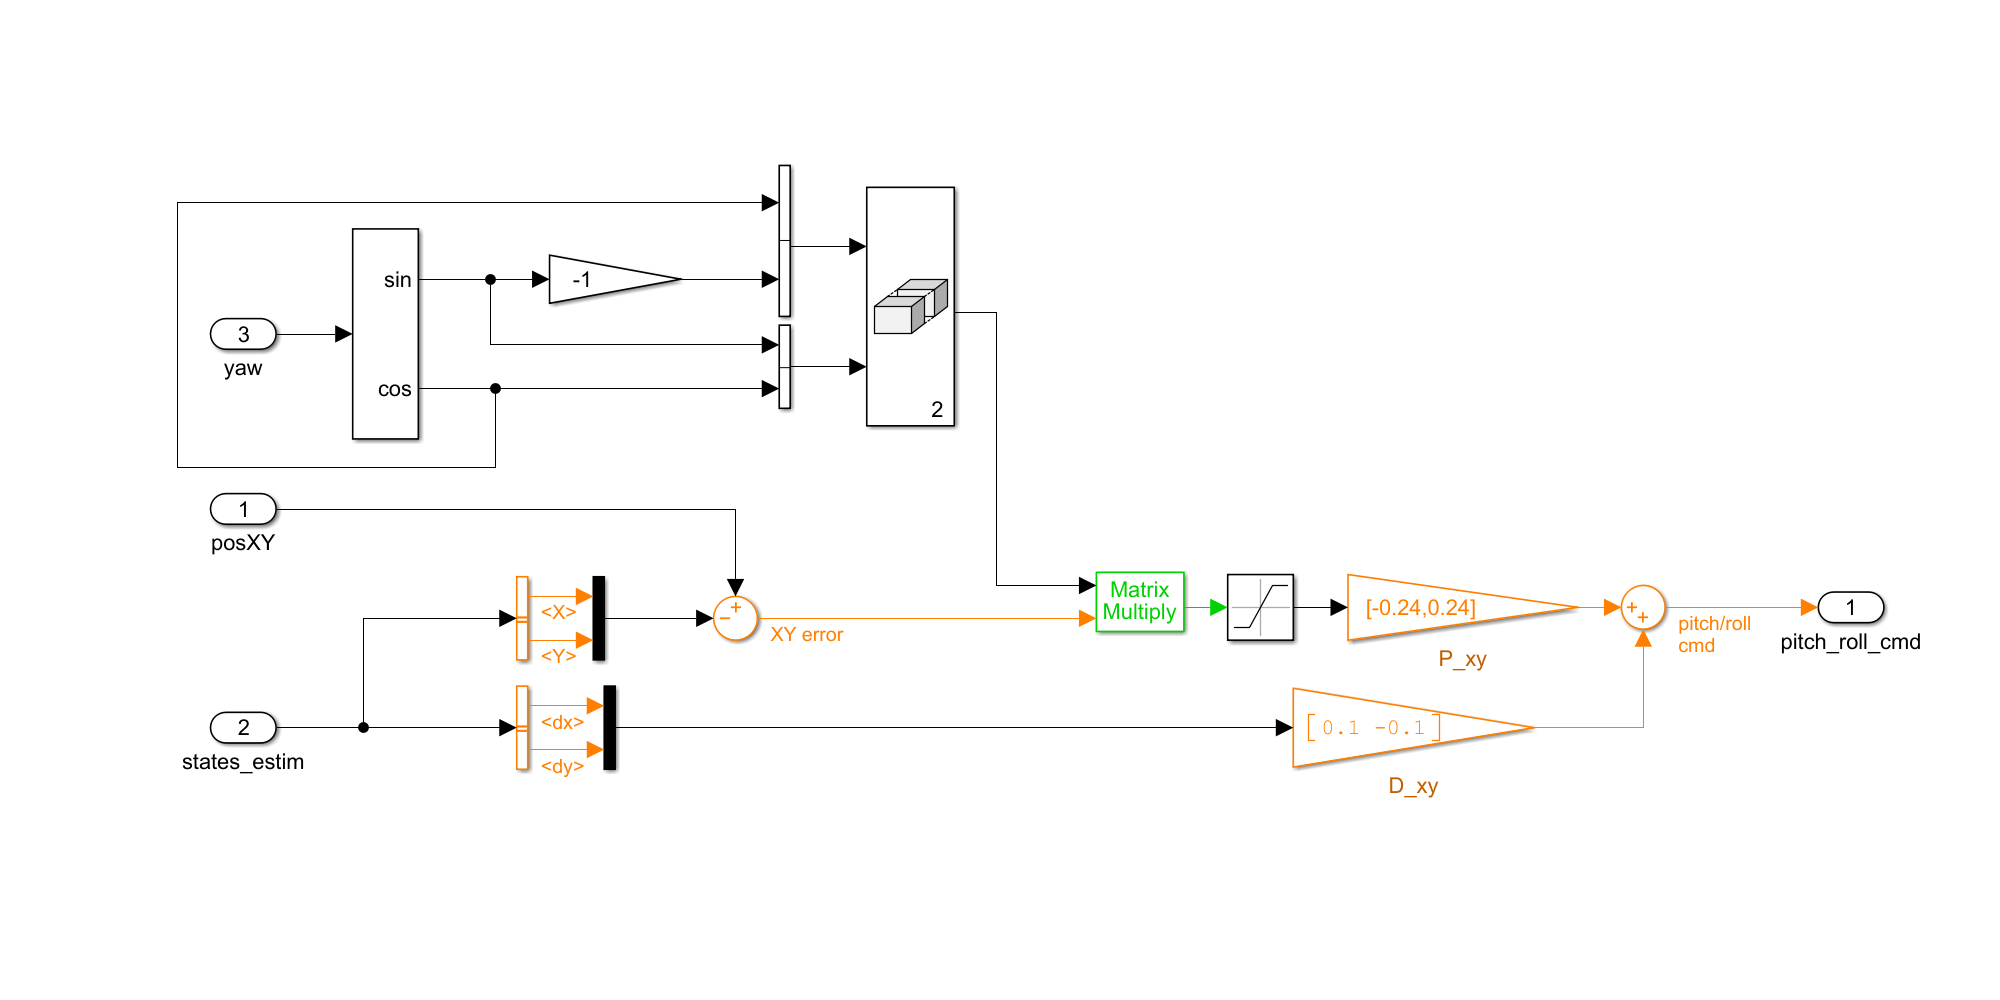
\includegraphics[width=0.8\textwidth]{flightControlSystem-controller-toReference}
	\caption{Estimador/Controlador de Atitude Primário}
	\centering
	\label{Estimador de Atitude}
\end{figure}

-Attitude - Controlador de atitude, tem como objetivo calcular os torques para controle de atitude do quadricóptero, e faz isso utilizando um controlador PID.

\begin{figure}[H]
	\centering
	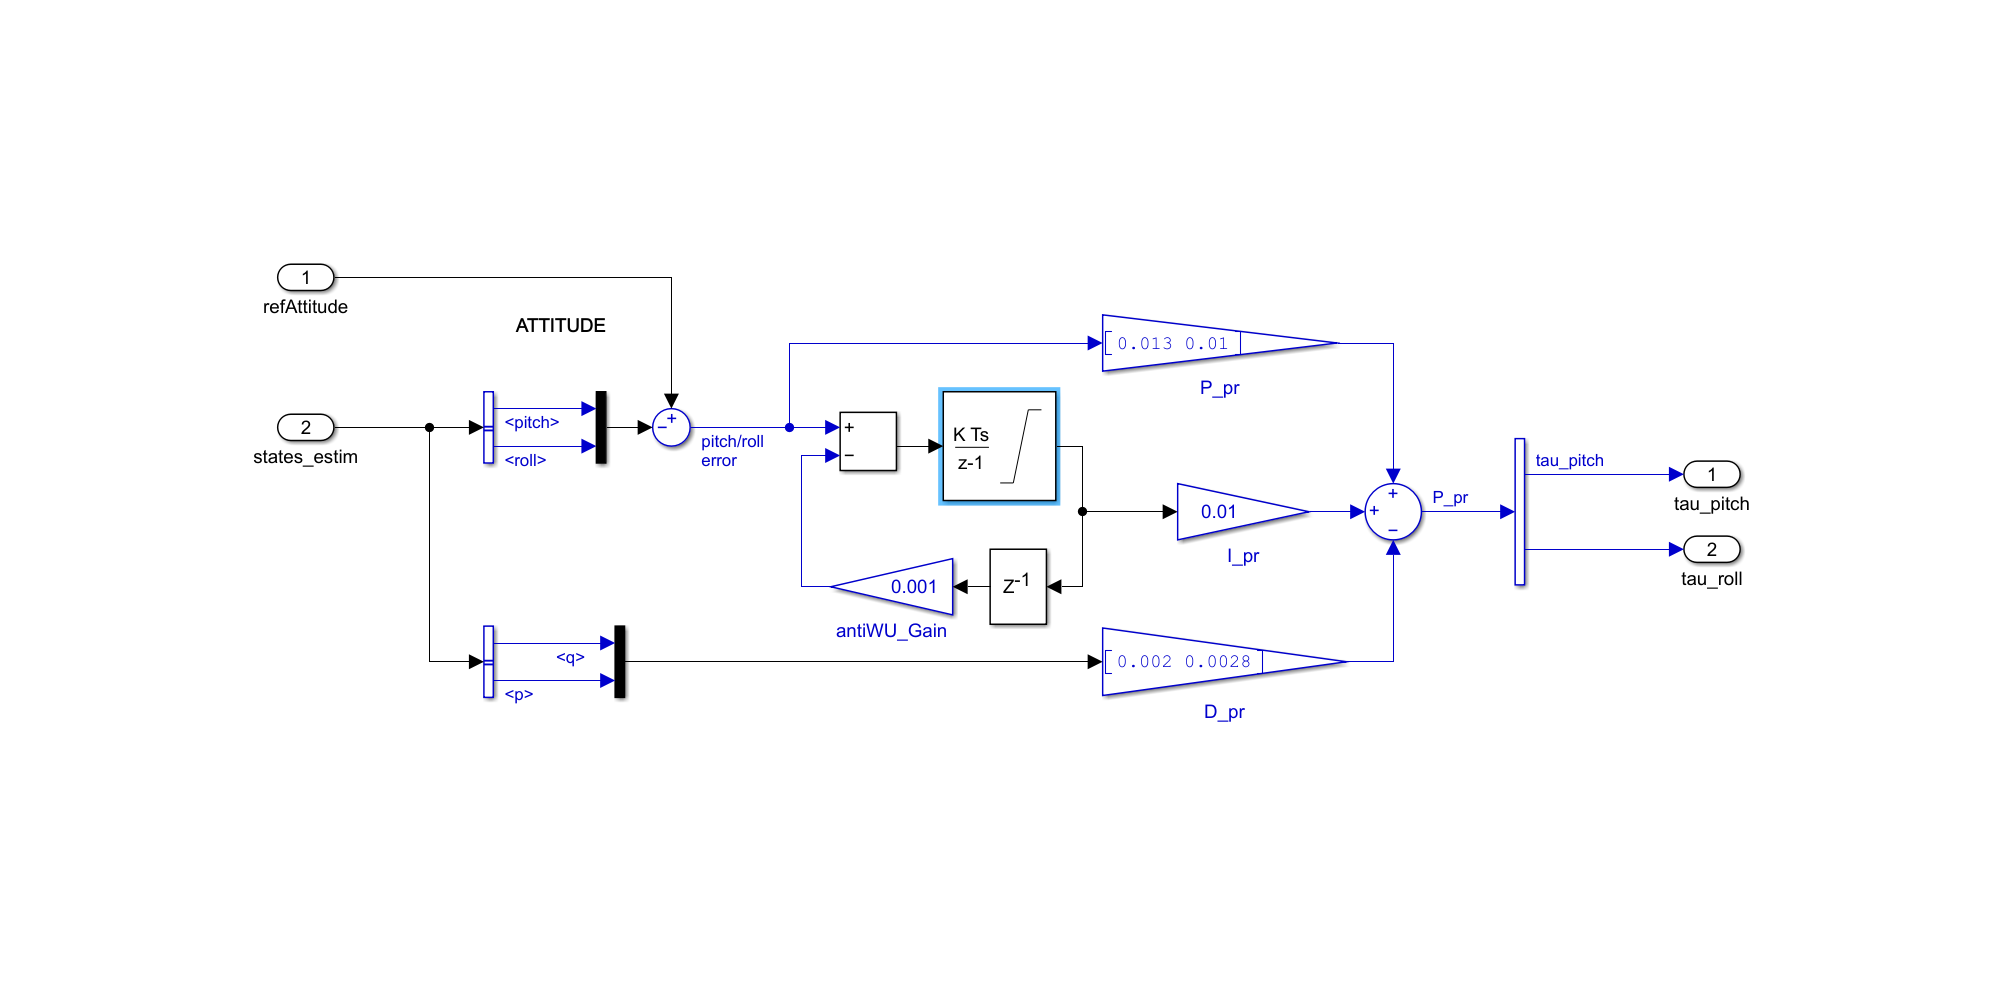
\includegraphics[width=1\textwidth]{flightControlSystem-controller-atitude}
	\caption{Controlador de Atitude}
	\centering
	\label{Controlador de Atitude}
\end{figure}


-Gravity feedforward/equilibrium thrust - Controlador de altitude,  tem como objetivo controlar a altitude do quadricóptero, e faz isso através de um controlador PD, calculando o empuxo necessário para atingir a altura desejada.

\begin{figure}[H]
	\centering
	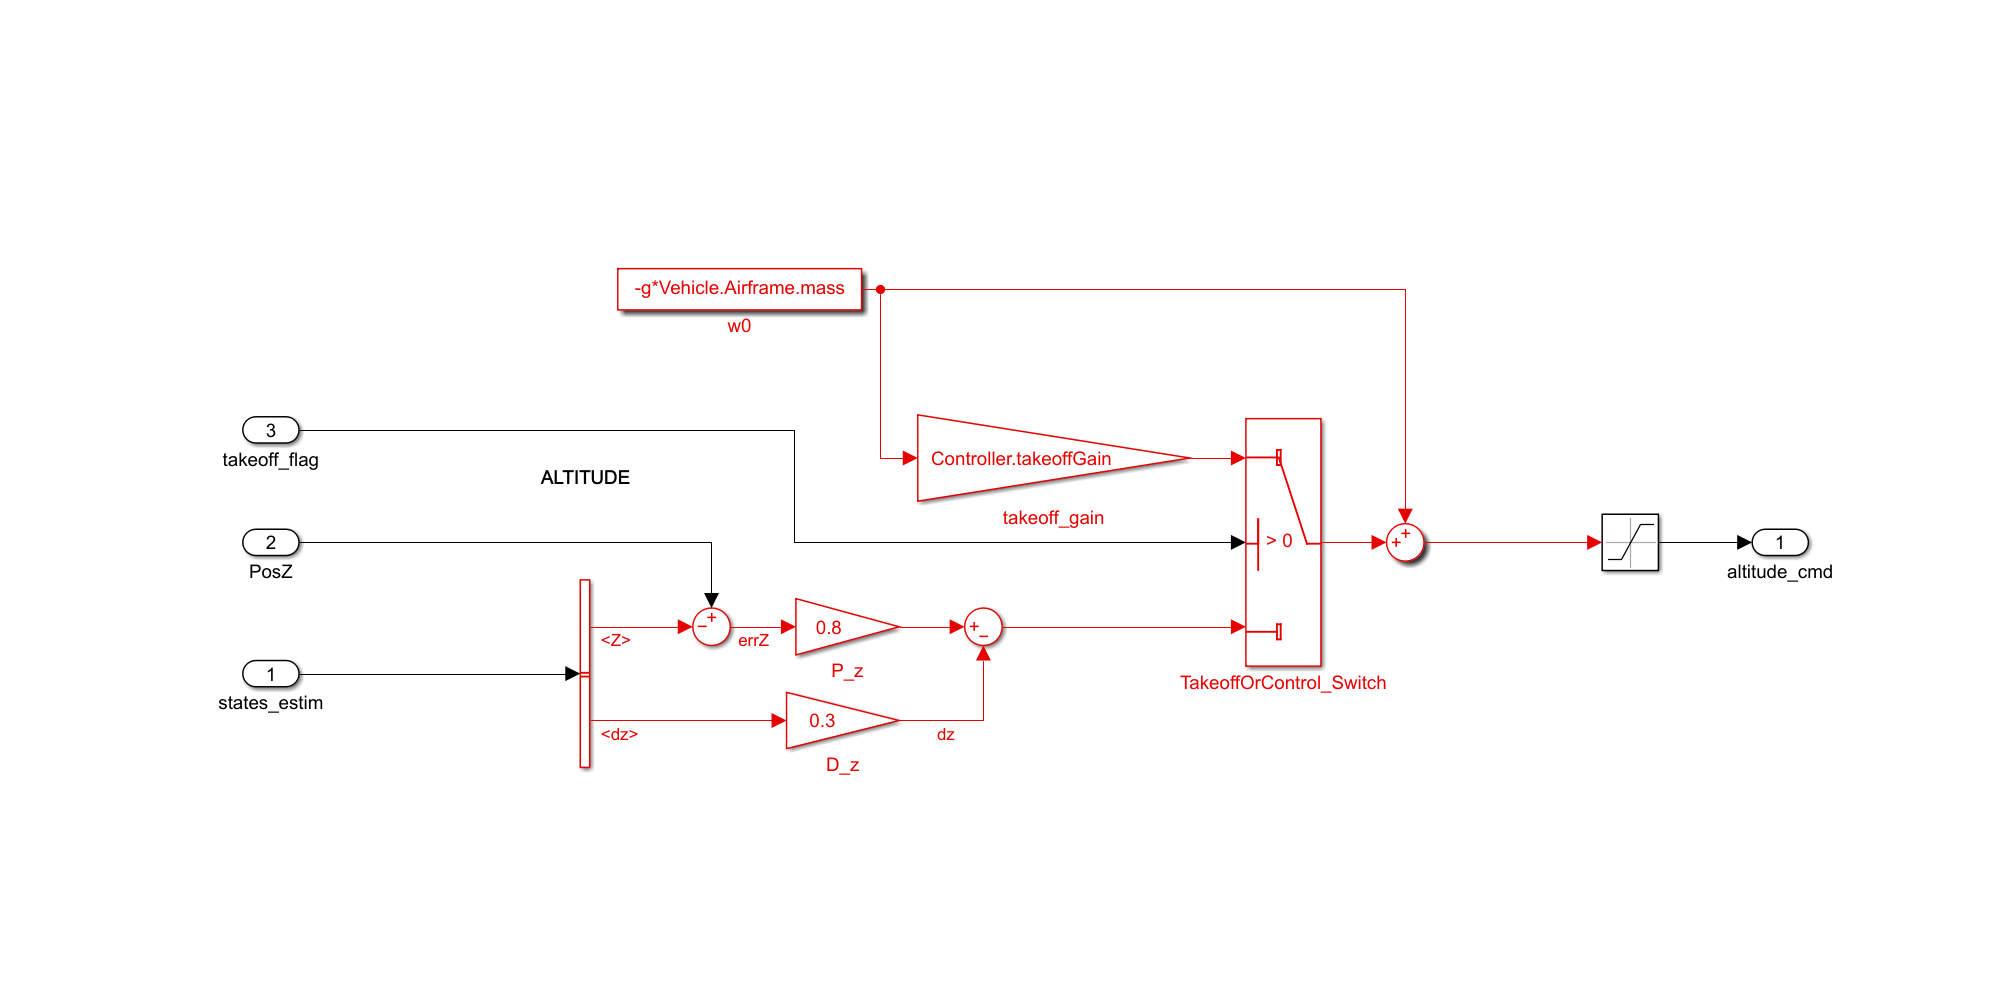
\includegraphics[width=0.8\textwidth]{flightControlSystem-controller-altitude}
	\caption{Controlador de Altitude}
	\centering
	\label{Controlador de Altitude}
\end{figure}

-Control Mixer - Junta as valores de torque necessário(torque de guinada, arfagem e rolamento) com o valor de empuxo para calcular o valor de empuxo necessário em cada motor. 

\begin{figure}[H]
	\centering
	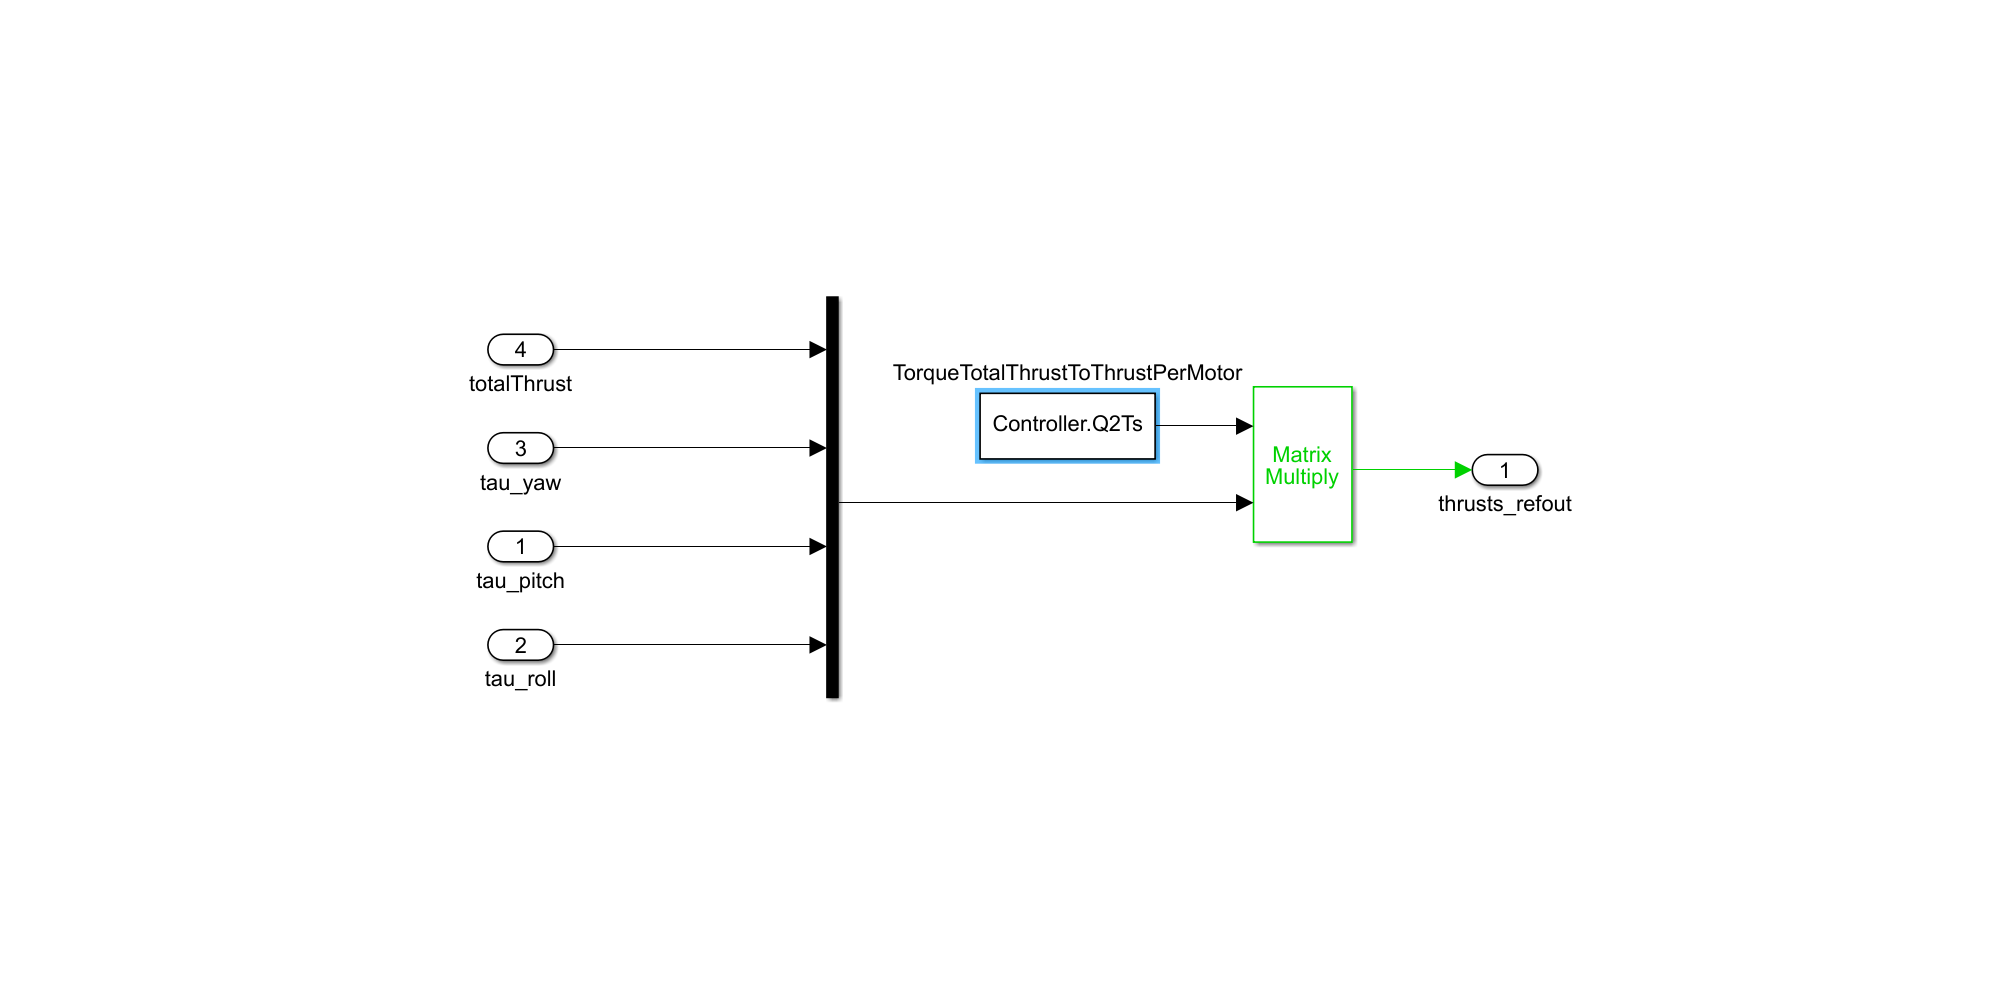
\includegraphics[width=1\textwidth]{flightControlSystem-controller-mixer}
	\caption{Agregador de Controle}
	\label{Agregador de Controle}
\end{figure}

-Thrusts To Motor Commands - Tem o objetivo de distribuir os empuxo necessário para os motores, transformando esses valores em comandos para os motores.

\begin{figure}[H]
	\centering
	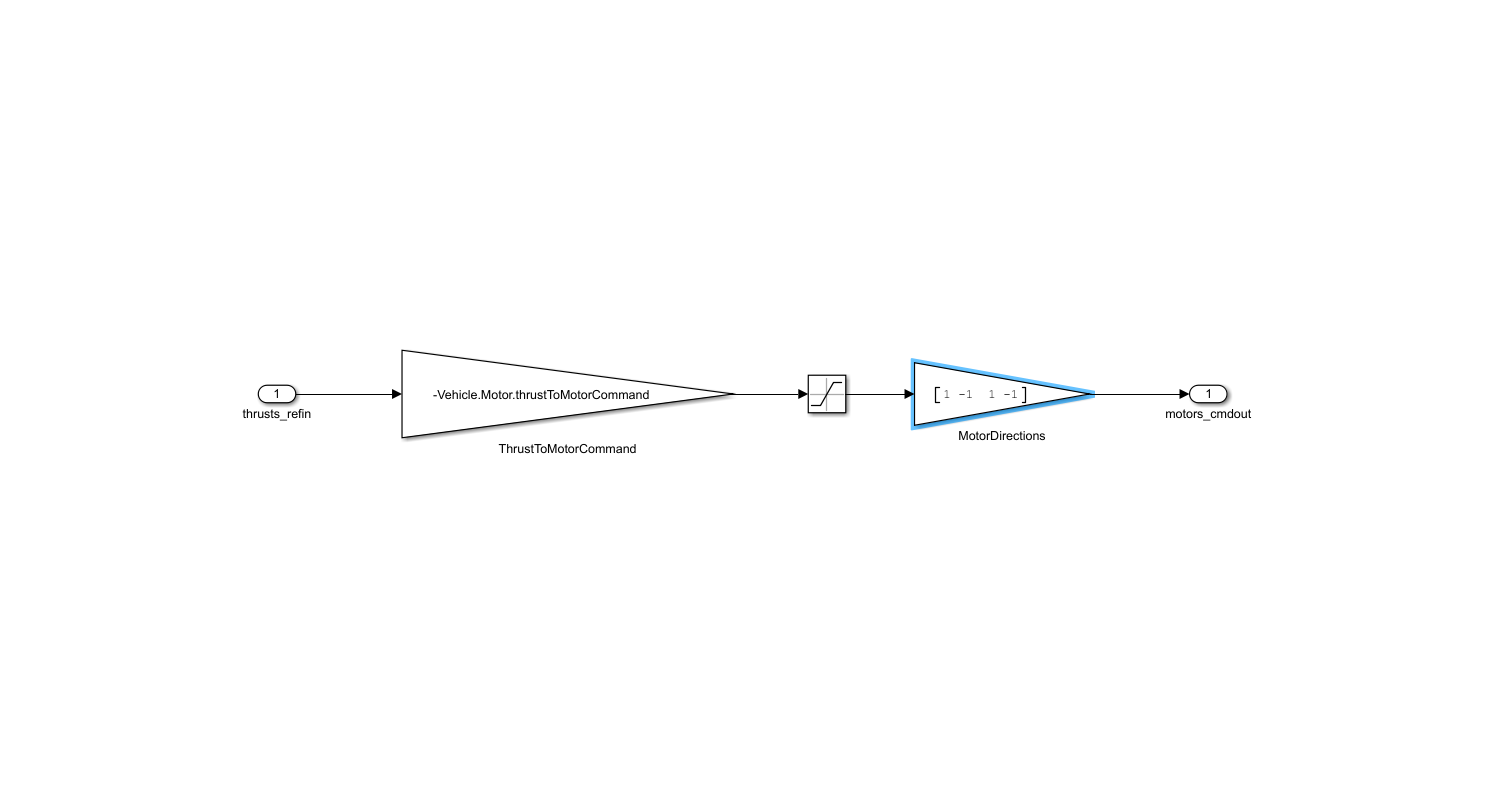
\includegraphics[width=0.8\textwidth]{flightControlSystem-controller-motorcmd}
	\caption{Transformador de Potência para Comandos de Motor}
	\centering
	\label{Transformador de Potência para Comandos de Motor}
\end{figure}


\section{Modelo do Quadricóptero no Matlab}

Nessa seção iremos analisar a planta do nosso sistema de controle, que no nosso caso, podemos nos referir como modelo dinâmico do quadricóptero. Na imagem abaixo podemos observar que temos duas opções de modelos para utilizar, um modelo linear e um modelo não linear, sendo que a alternancia entre modelos pode ser feita de forma simples alterando a variável \textit{VSSVEHICLE}.

Assim, iremos analisar a construção dos dois modelos e explicitar suas diferenças.

\begin{figure}[H]
	\centering
	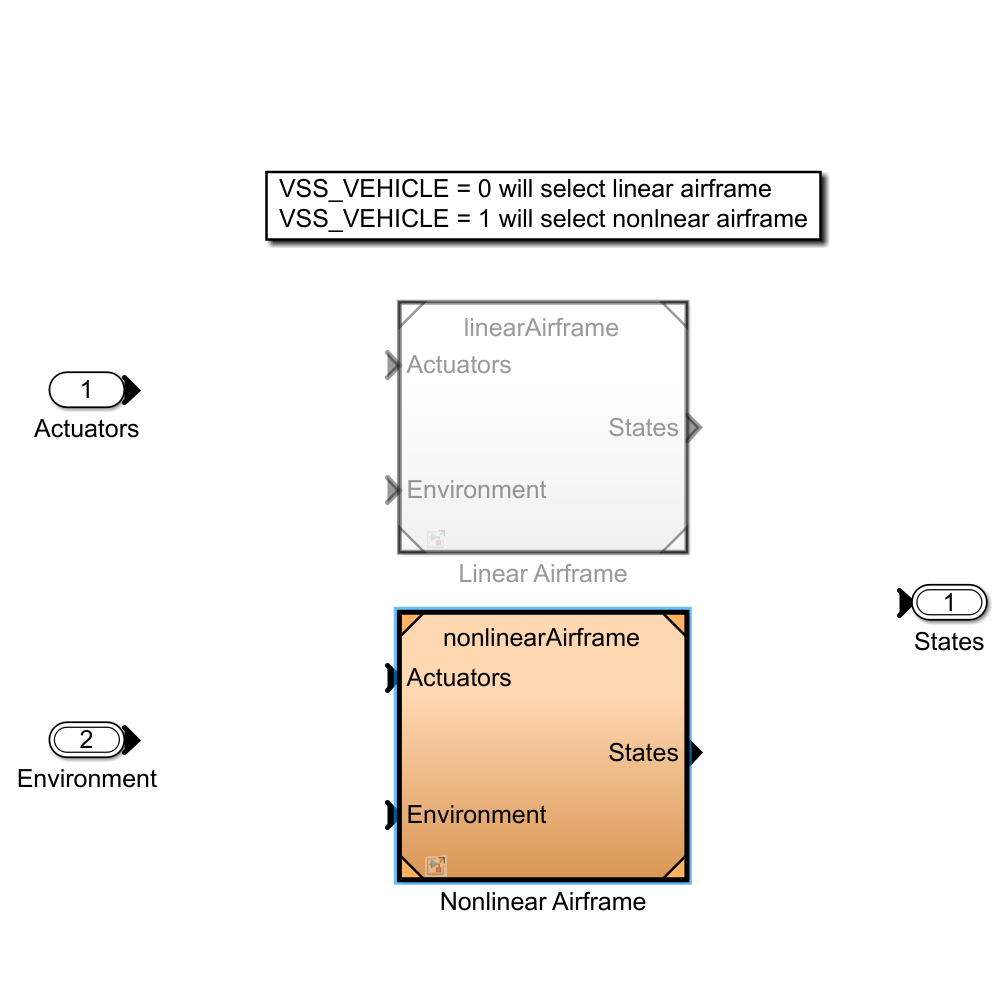
\includegraphics[width=1\textwidth]{asbQuadcopterProject - plant.png}
	\caption{Modelo dinâmico do quadricóptero}
	\centering
	\label{Modelo dinâmico do quadricóptero}
\end{figure}

-NonLinear Airframe - O modelo não linear do quadricóptero temos 2 subsistemas(blocos) importantes, o \textit{modelo AC}, que tem o papel de calcular as forças e momentos aerodiâmicos, sendo este o modelo dos atuadores e de como as perturbações do ambiente afetam o sistema e o \textit{6DOF(Ângulos de Euler)}, que recebe as forças e torques calculadas no \textit{modelo AC}, e integra as equações de movimento para obter os estados do quadricópteroa cada instante. O bloco 6DOF é uma representação de um corpo rígido que vêm do pacote  \textit{Aerospace blockset} do matlab e podemos selecionar o método de análise entre quaterinions e angulos de Euler.

\begin{figure}[H]
	\centering
	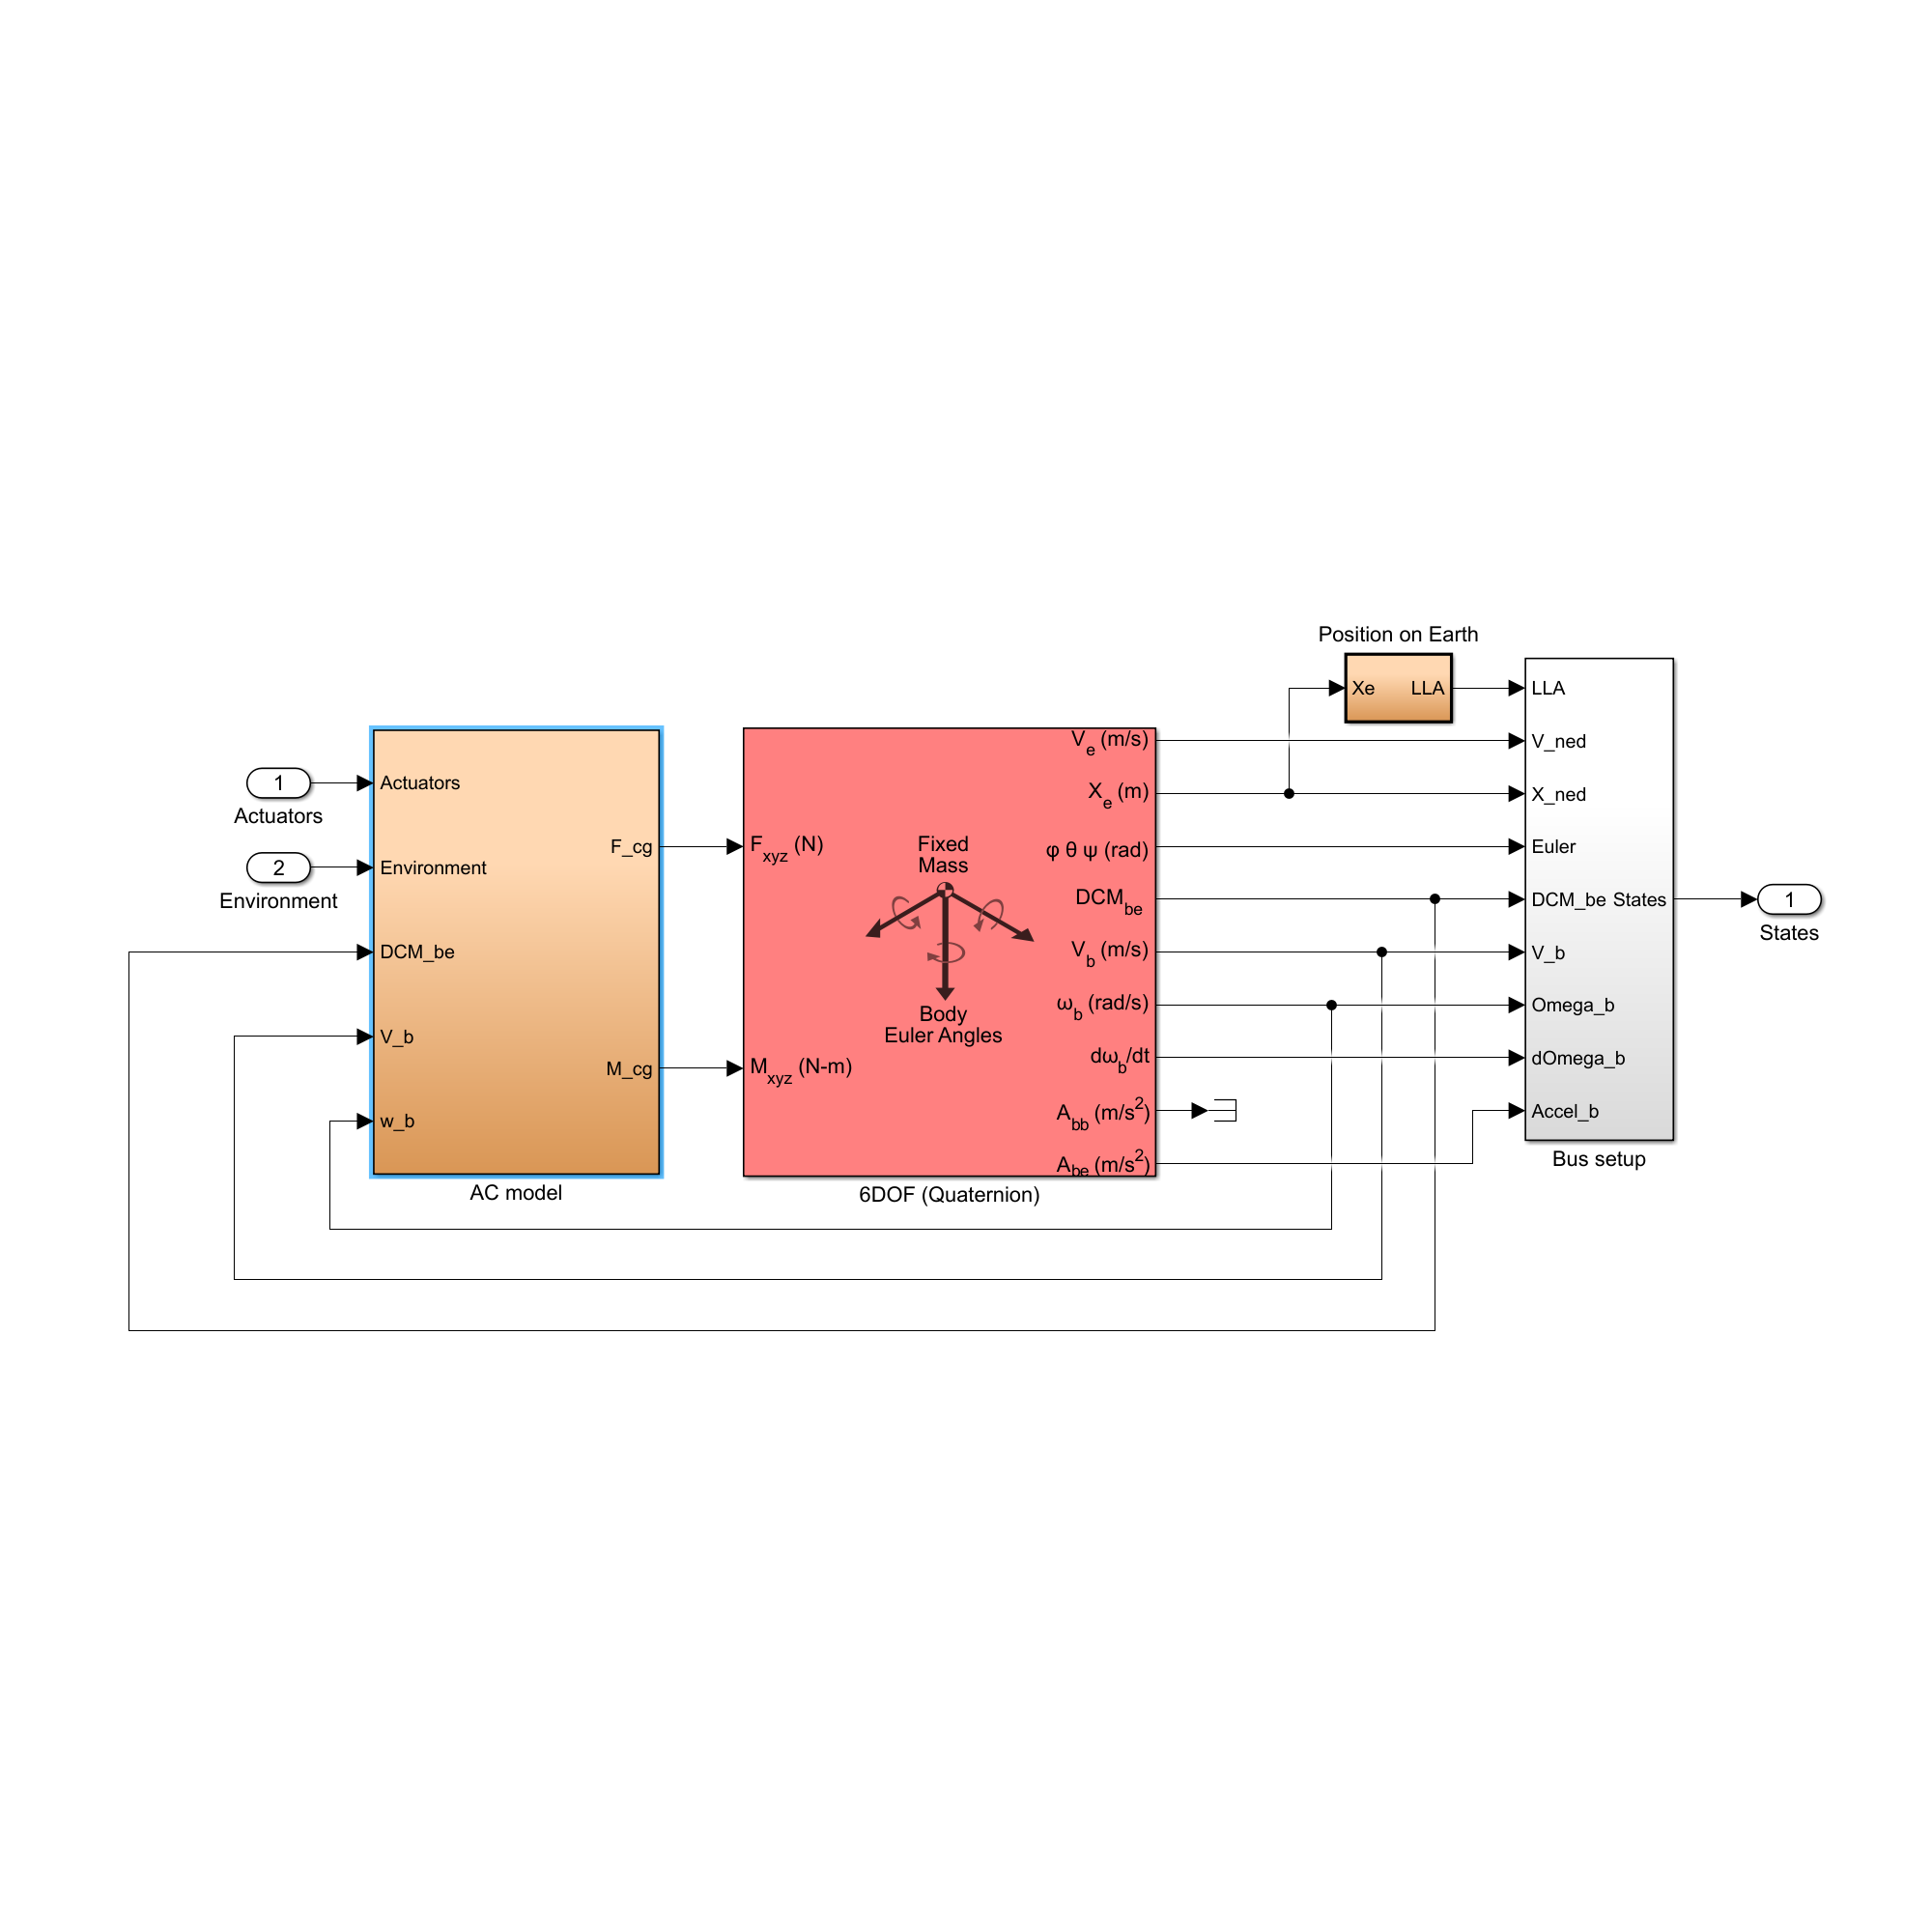
\includegraphics[width=1\textwidth]{asbQuadcopterProject - plant - nonLinear.png}
	\caption{Modelo não linear do Quadricóptero}
	\centering
	\label{Modelo não linear do Quadricóptero}
\end{figure}


\begin{figure}[H]
	\centering
	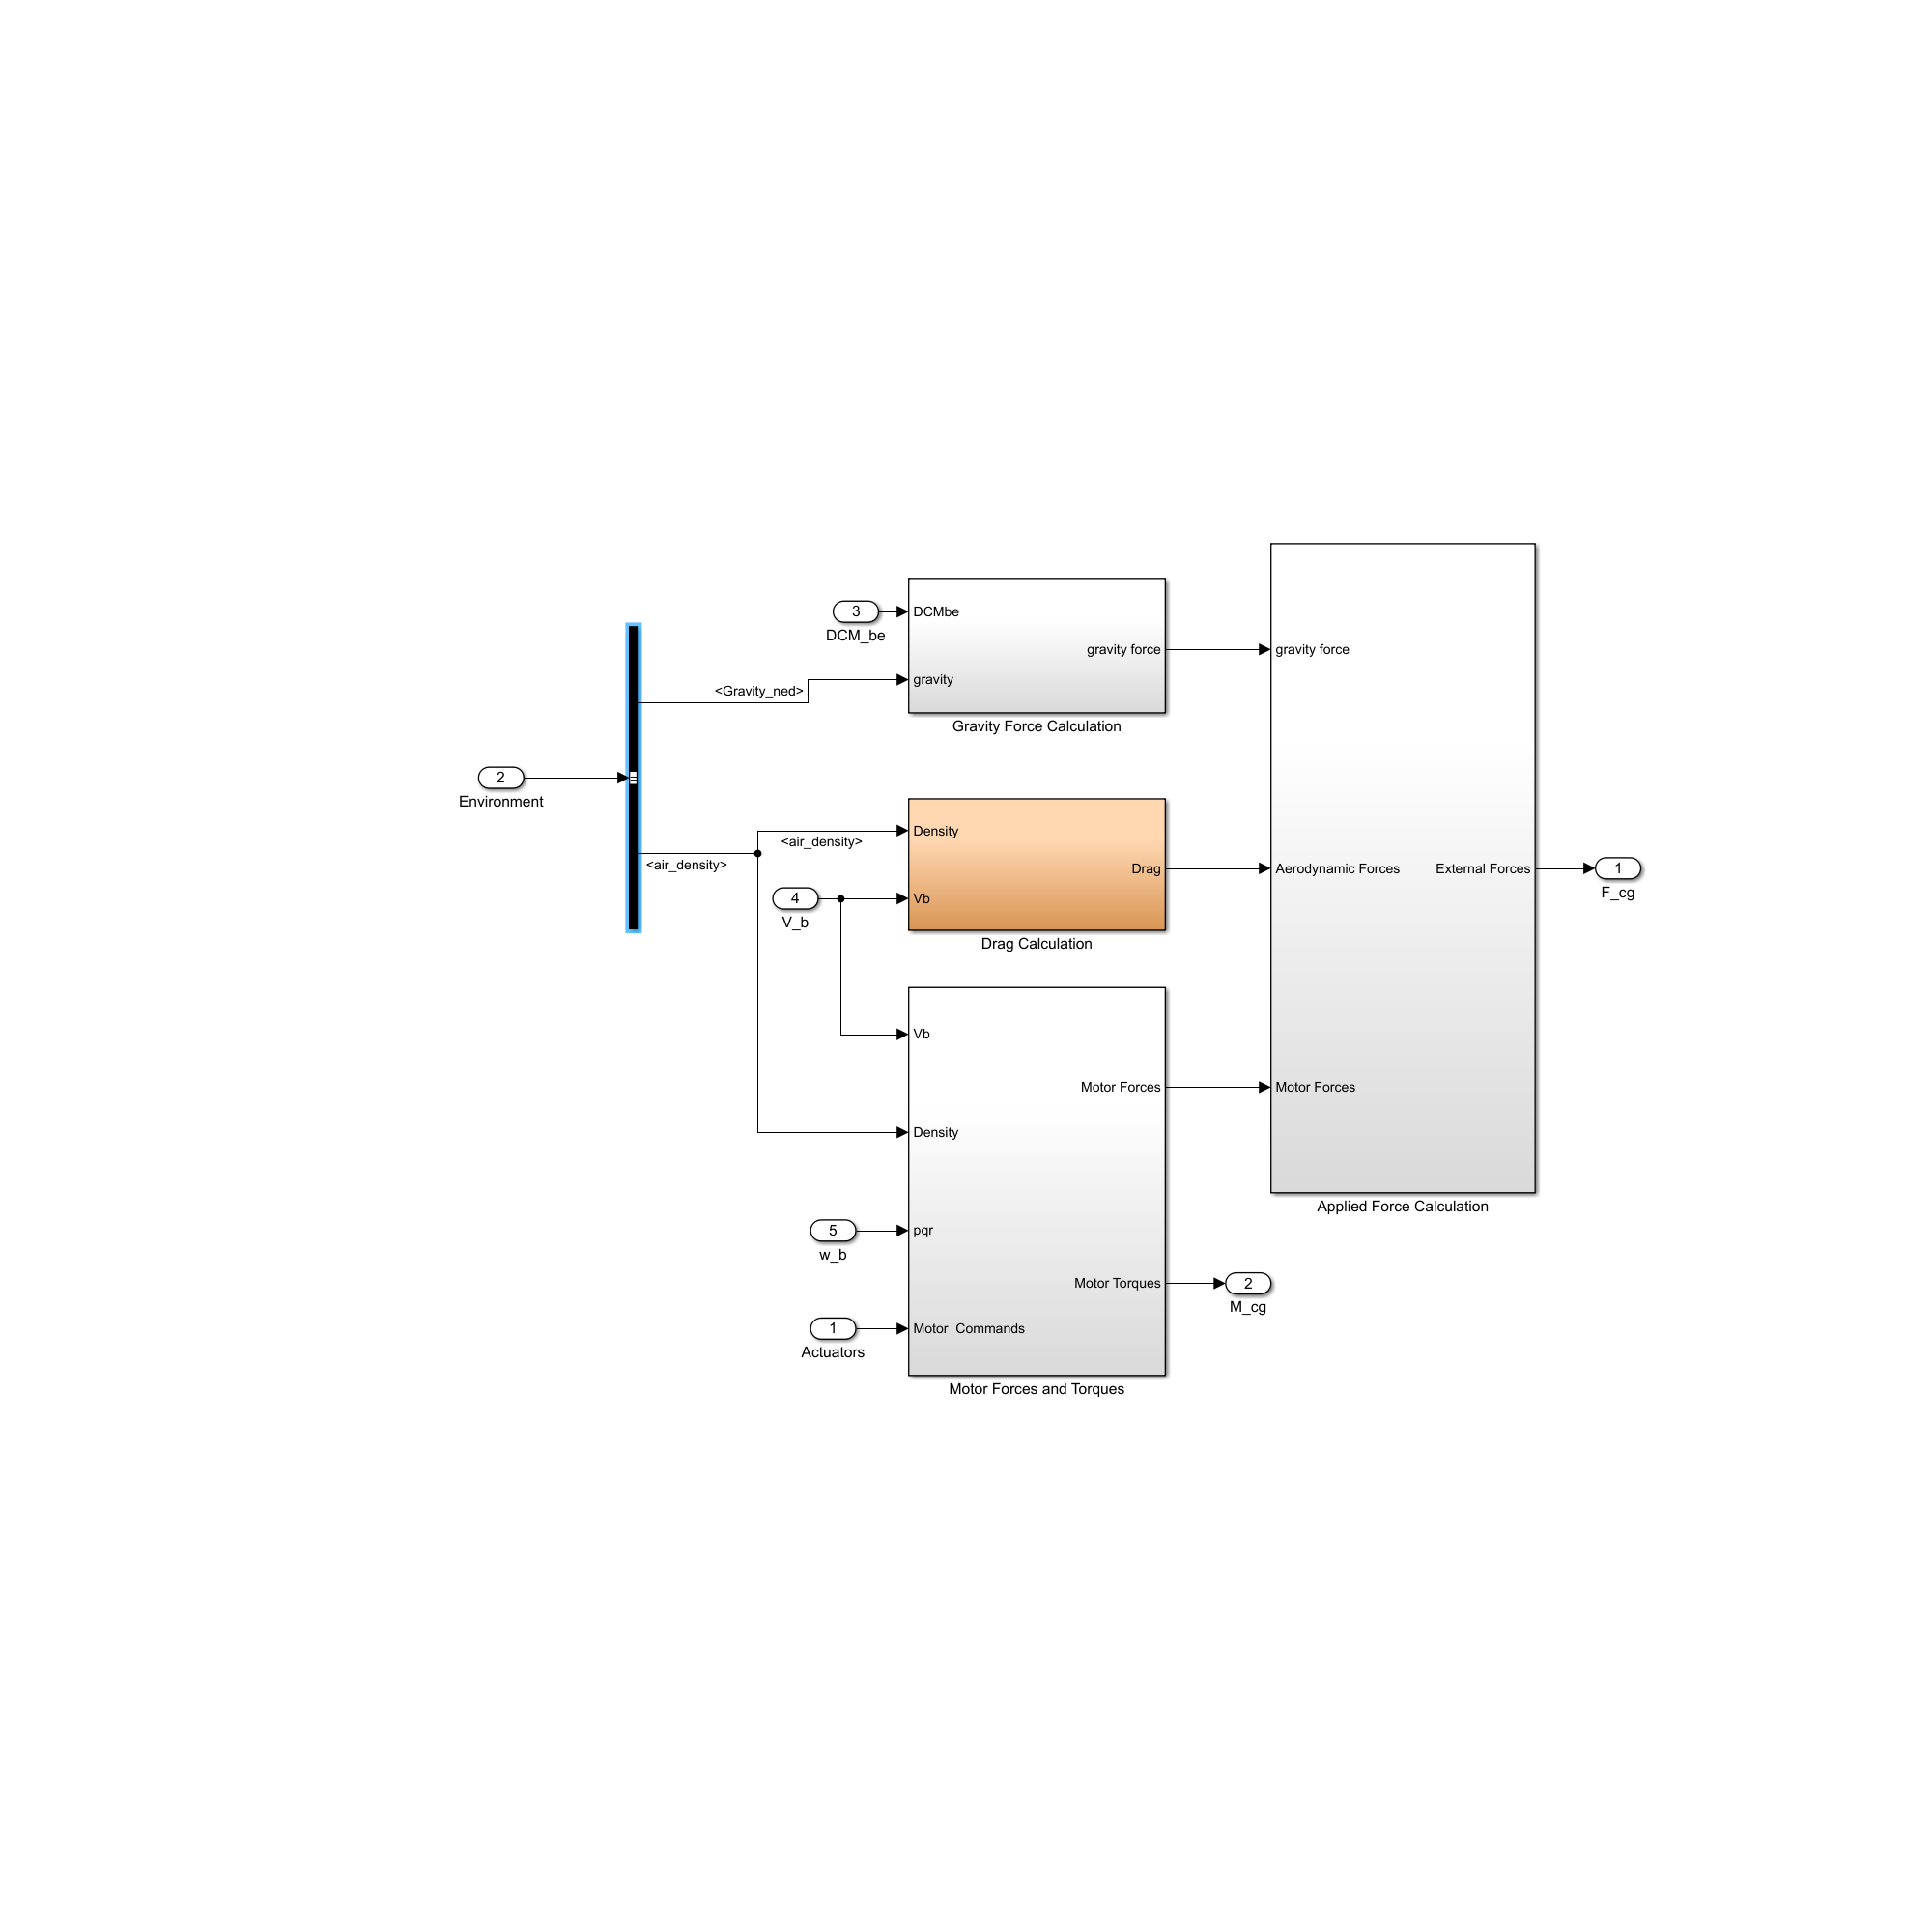
\includegraphics[width=1\textwidth]{asbQuadcopterProject - plant - nonLinear-ac-model.png}
	\caption{Modelo AC}
	\centering
	\label{Modelo AC}
\end{figure}



-Linear Airframe - O modelo linear nesse caso é o modelo não linear linearizado utilizando  Simulink® Control Design™, sendo que apesar do modelo linear ser menos preciso que o modelo não linear, ele é importante para podermos aplicar técnicas de otimização de controle linear.

\begin{figure}[H]
	\centering
	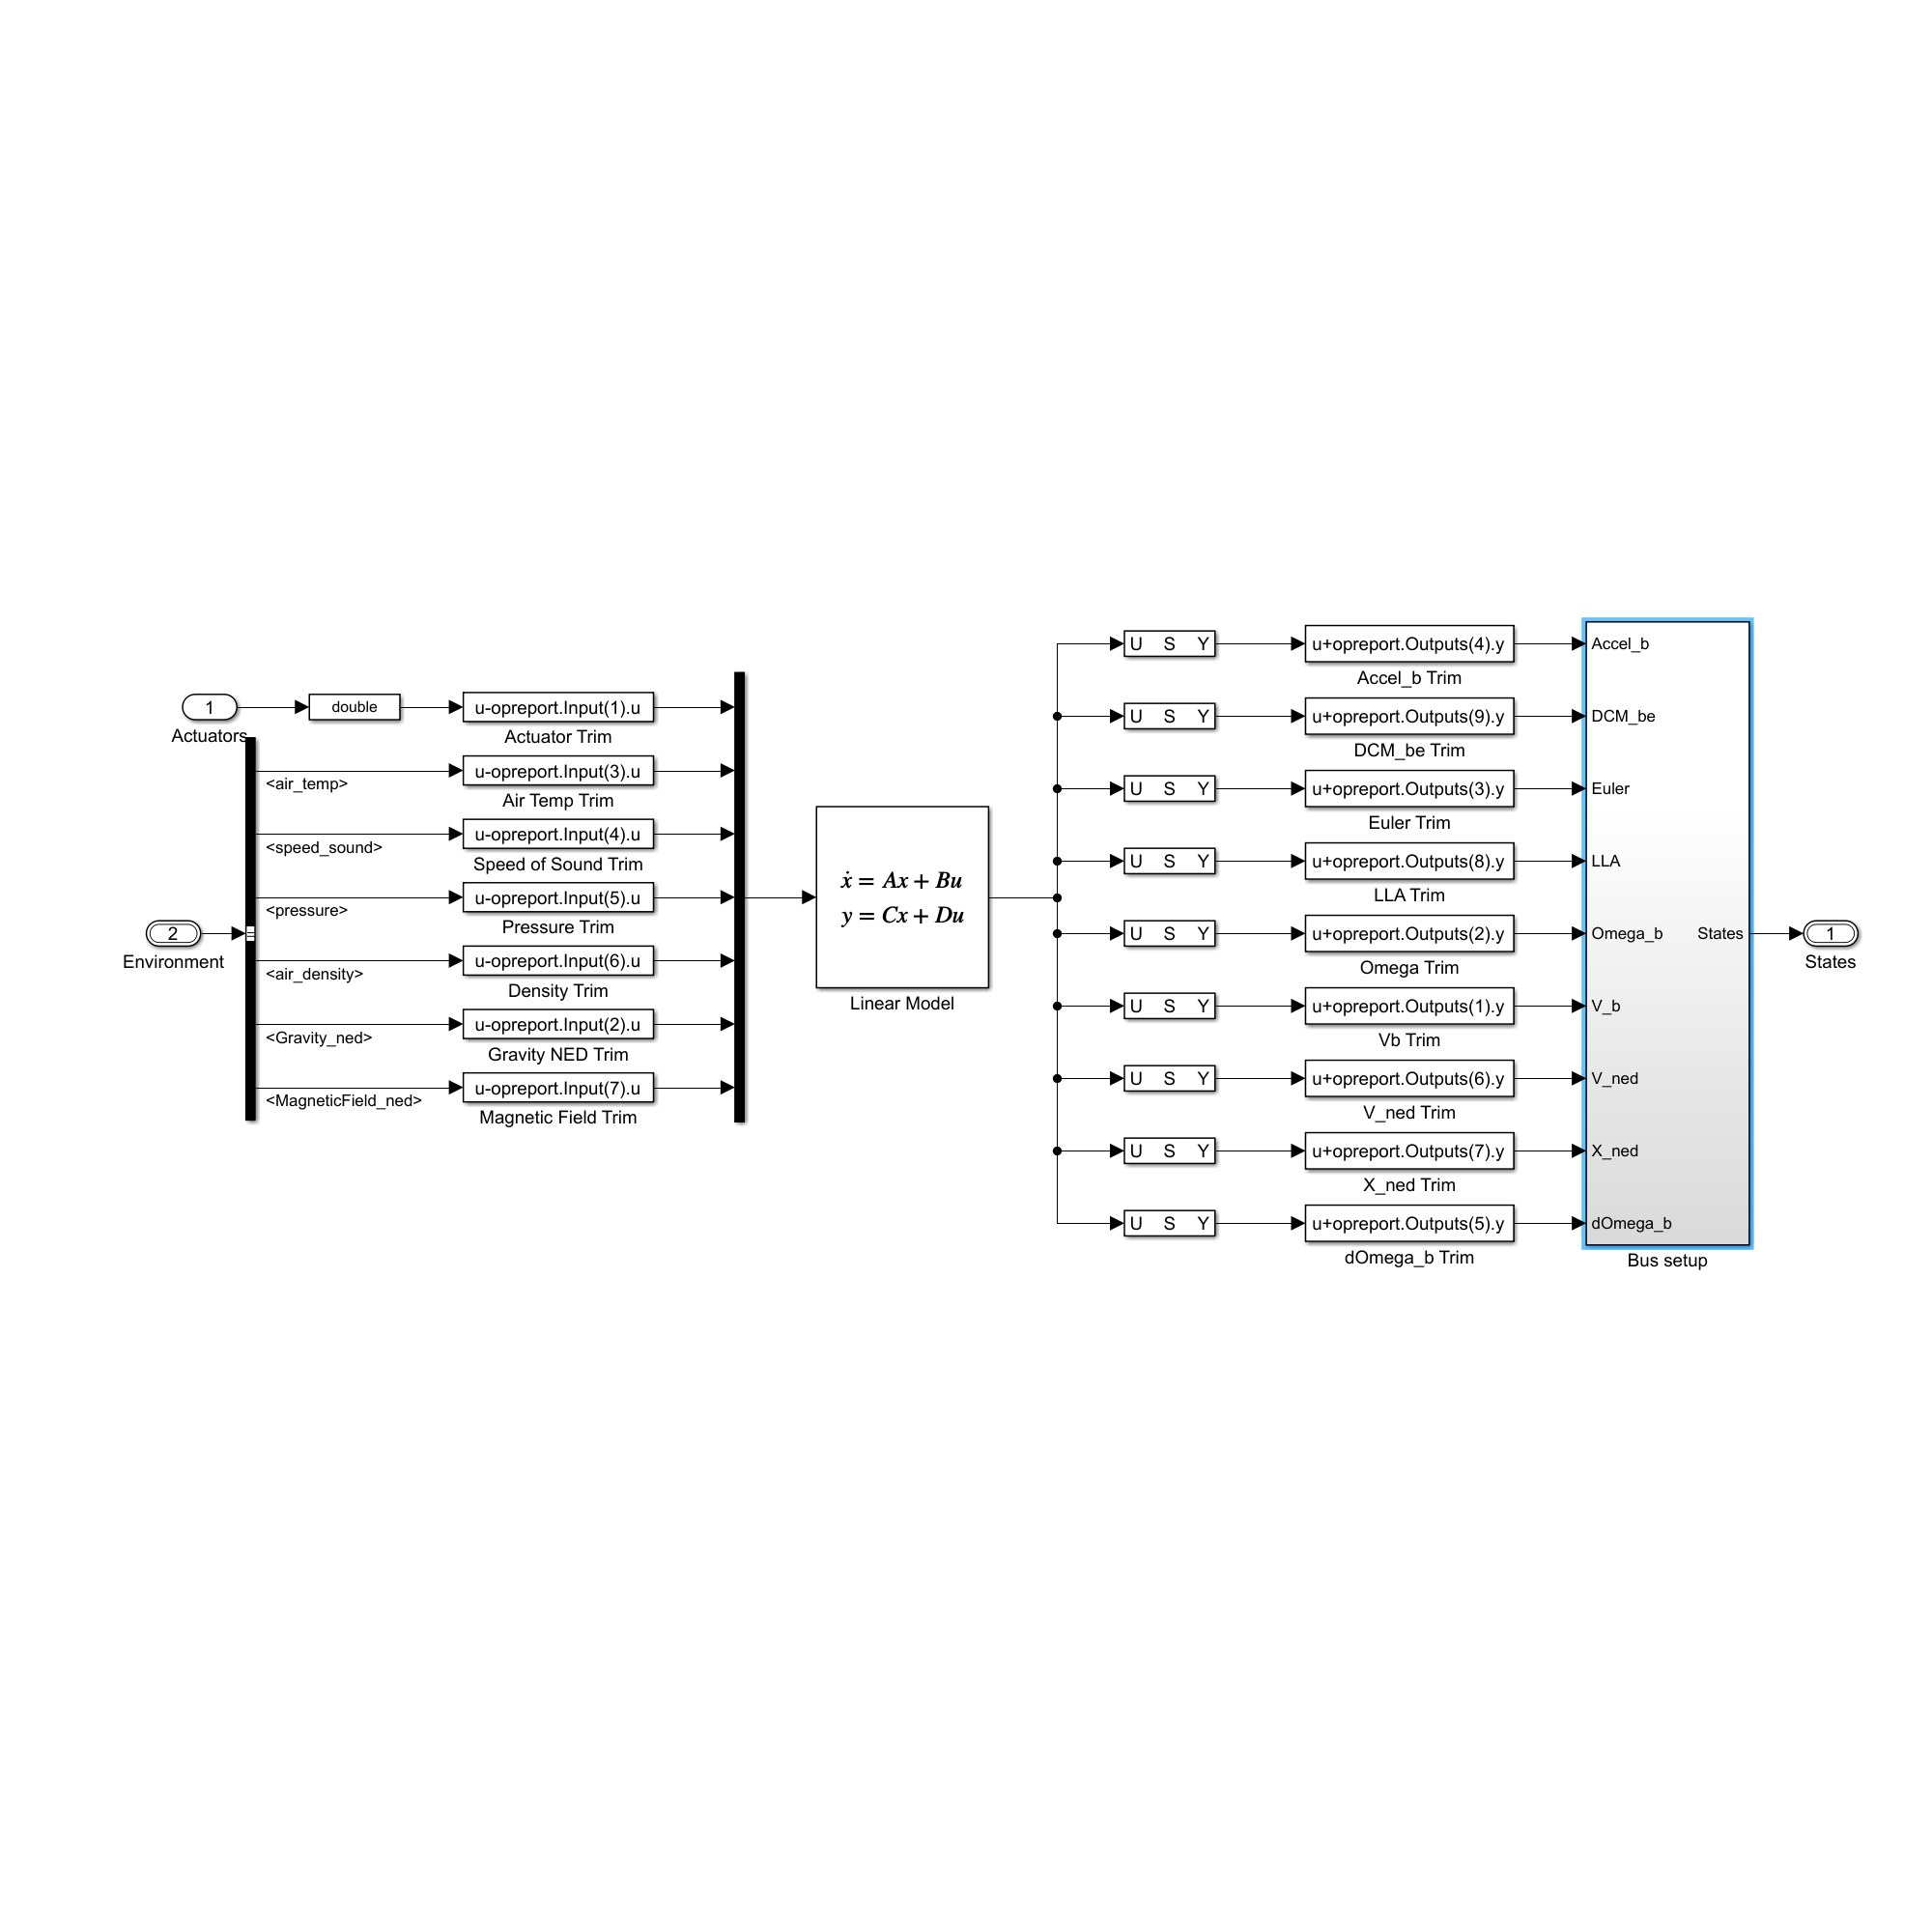
\includegraphics[width=1\textwidth]{asbQuadcopterProject - plant - linear.png}
	\caption{Modelo linear do Quadricóptero}
	\centering
	\label{Modelo linear do Quadricóptero}
\end{figure}
%---------------------------------------------------------------------
% INDICE REMISSIVO
%---------------------------------------------------------------------
\phantompart
\printindex
%---------------------------------------------------------------------
